% 前所未有简单地,开始你的 LaTeX 之旅

%%%%%%%%%%%%%%%%%%%%%%%%%%%%%%%%%%%%%%%%%%%%%%%%%%%%%%%%%%%%%%%%%%%%%%%%%
% [页面选项]
%
% 字号选项:    11pt是字号,比较适合电子印刷品和纸质印刷品
% 字体选项:    不填写 - 默认为 Modern (别忘了连逗号一起删了)
%			  times - Times New Roman
%			  sans - Sans Serif 字体(黑体)
% oneside:    代表单面,一般单侧用于电子印刷品
% 		      可以改成 twoside,一般用于双面纸质印刷
% openright:  双面打印的情况下,纸质印刷品要求新的一章从奇数页开始
% hardcopy:   打印机打印选项,带有此选项将去除logo颜色以及代码颜色,更适合黑白印刷
%			  使用彩色或者电子版请去除此选项
%			  也可以改为 editing ,颜色讲和 sublime3 的 Mariana 颜色主题一致,减小写作时的文本对比度
%		          让你以最舒适的方式书写
% heading:    页面带有页眉
\documentclass[11pt,times,oneside,openright]{eeereport}
%%%%%%%%%%%%%%%%%%%%%%%%%%%%%%%%%%%%%%%%%%%%%%%%%%%%%%%%%%%%%%%%%%%%%%%%%

%%%%%%%%%%%%%%%%%%%%%%%%%%%%%%%%%%%%%%%%%%%%%%%%%%%%%%%%%%%%%%%%%%%%%%%%%
% [封面选项]
%
% title:    文章主标题,不可以省略
% subtitle: 副标题,可以省略,但不可以删除
% covercontent: 封面信息,可以在其内部添加或者删除 \converline 来添加或者删除一行
%    coverline{项目}{项目内容},可以自由添加各种内容
%
\title{Domain Adaptation for Medical Image Segmentation on Lung Tumour Datasets}
\subtitle{}
\covercontent{
	\coverline{Author}{Zirui Zhou}
	\coverline{Student ID}{1927924}
	\coverline{Supervisor}{Erick Purwanto}
	\coverline{Accessor}{Jianjun Chen}
}
%%%%%%%%%%%%%%%%%%%%%%%%%%%%%%%%%%%%%%%%%%%%%%%%%%%%%%%%%%%%%%%%%%%%%%%%%


%%%%%%%%%%%%%%%%%%%%%%%%%%%%%%%%%%%%%%%%%%%%%%%%%%%%%%%%%%%%%%%%%%%%%%%%%
% 页面设定
% 如果在前面设定了需要页面,请去掉下面三个的注释,然后分别进行定义,如果不定义,
% LaTeX 会自动使用章节名称来进行页面定义
%\lhead{} 
%\chead{} 
%\rhead{}
%%%%%%%%%%%%%%%%%%%%%%%%%%%%%%%%%%%%%%%%%%%%%%%%%%%%%%%%%%%%%%%%%%%%%%%%%
\usepackage{listings}
\usepackage{color}

\definecolor{dkgreen}{rgb}{0,0.6,0}
\definecolor{gray}{rgb}{0.5,0.5,0.5}
\definecolor{mauve}{rgb}{0.58,0,0.82}

\lstset{frame=tb,
  language=Python,
  aboveskip=3mm,
  belowskip=3mm,
  showstringspaces=false,
  columns=flexible,
  basicstyle={\small\ttfamily},
  numbers=none,
  numberstyle=\tiny\color{gray},
  keywordstyle=\color{blue},
  commentstyle=\color{dkgreen},
  stringstyle=\color{mauve},
  breaklines=true,
  breakatwhitespace=true,
  tabsize=2,
  numbers=left,                    
  numbersep=5pt, 
}

\usepackage[parfill]{parskip}

\usepackage[numbers]{natbib}

\usepackage{multirow}

\usepackage{tabularx}

\usepackage[toc]{appendix}

\usepackage[xindy={glsnumbers=false}, nonumberlist, nopostdot, nogroupskip]{glossaries}

\usepackage{hyperref}

\setglossarystyle{long}
\renewcommand{\glsnamefont}[1]{\textbf{#1}}

\makeglossaries
\newacronym{unet}{U-Net}{Convolutional Networks for Biomedical Image Segmentation}
\newacronym{ct}{CT}{Computed Tomography}
\newacronym{gan}{GAN}{Generative Adversarial Network}
\newacronym{vae}{VAE}{Variational Autoencoder}
\newacronym{rider}{RIDER}{The Reference Image Database to Evaluate Therapy Response}
\newacronym{tcia}{TCIA}{The Cancer Imaging Archive}
\newacronym{nsclc}{NSCLC}{Non-Small Cell Lung Cancer}
\newacronym{msd}{MSD}{Medical Segmentation Decathlon}
\newacronym{nifti}{NIfTI}{Neuroimaging Informatics Technology Initiative}
\newacronym{dicom}{DICOM}{Digital Imaging and Communications in Medicine}
\newacronym{mri}{MRI}{Magnetic Resonance Imaging}
\newacronym{dcmqi}{DCMQI}{DICOM for Quantitative Imaging}
\newacronym{cnn}{CNN}{Convolutional Neural Network}
\newacronym{vit}{ViT}{Vision Transformer}
\newacronym{nlp}{NLP}{Natural Language Processing}
\newacronym{msa}{MSA}{Multihead Self-attention}
\newacronym{unetr}{UNETR}{UNet Transformer}
\newacronym{uda}{UDA}{Unsupervised Domain Adaptation}
\newacronym{kl}{KL}{Kullback–Leibler}
\newacronym{sclc}{SCLC}{Small Cell Lung Cancer}
\newacronym{sifa}{SIFA}{Synergistic Image and Feature Adaptation}


\setlength\LTleft{0pt}
\setlength\LTright{0pt}
\setlength\glsdescwidth{0.8\hsize}

\begin{document}
% set line spacing to 1.5B
\baselineskip = 17pt
\pagenumbering{Alph}
\begin{titlepage}
% 不要编译!该文件已经包含在 report.tex 里了
\thispagestyle{empty}
\newcommand\nbvspace[1][3]{\vspace*{\stretch{#1}}}
\newcommand\nbstretchyspace{\spaceskip0.5em plus 0.25em minus 0.25em}
\newcommand{\nbtitlestretch}{\spaceskip0.6em}
\newcommand{\psubtitle}[1]{\LARGE\textbf{{#1}}\\\normalsize}
\newcommand{\ptitle}[1]{\huge\textbf{{#1}}\\\normalsize}

\begin{center}
\nbvspace[0.5]
\begin{figure}[h]
\centering
\includegraphics[width=10cm]{\logofile}
\label{fig:logo}
\end{figure}
%\psubtitle{Experimental Report}
\nbvspace[1]
\ptitle{\rtt}
\nbvspace[0.5]
\psubtitle{\srtt}
\nbvspace[1]

\end{center}
\begin{flushleft}

\begin{table}[!hbp]
\centering
\begin{tabular}{p{2.5cm} p{7cm}}   \\
  \cct
 \end{tabular}
\end{table}
\normalsize
\nbvspace[0.5]
\end{flushleft}

\newpage
\thispagestyle{empty}
\end{titlepage}

\frontmatter

\tableofcontents
\addcontentsline{toc}{chapter}{Contents}

\listoffigures
\listoftables

\printglossary[title=Acronyms]
%%%%%%%%%%%%%%%%%%%%%%%%%%%%%%%%%%%%%%%%%%%%%
% 摘要部分 Abstract
%%%%%%%%%%%%%%%%%%%%%%%%%%%%%%%%%%%%%%%%%%%%%
\chapter{Abstract}
Over the past few decades, advances have been made in the classification, diagnosis and treatment of lung cancer in many ways. Machine learning-based lung cancer prediction models such as semantic segmentation have been proposed to assist clinicians in the management of incidentally detected or screened-out indeterminate lung nodules. Semantic segmentation transforms raw medical images into clinically relevant, spatially structured information, such as outlining tumour boundaries and is an essential prerequisite for abundant clinical applications. However, the normal segmentation models may not have qualified performance, due to the lack of labelled medical imaging datasets. Domain adaptation can be introduced to finetune the target datasets on one pre-trained model for better accuracy. This project focuses on applying a segmentation and shaping model based domain adaptation framework with 3D \acrshort{unet} and \acrshort{unetr} as its backbone. Experimental results demonstrate that the Dice gap between a certain method and direct tests is around 2\% in most cases, where three datasets are imported including \acrshort{msd}, \acrshort{rider}, and \acrshort{nsclc}. Domain adaptation significantly improves the performance on the small dataset \acrshort{nsclc} of models pre-trained on the large dataset \acrshort{rider}. In addition, the 3D \acrshort{unet} with simple network architecture trained on the relatively abundant datasets \acrshort{rider} reaches the highest scores among the current results.

\textbf{Key Words:} Deep Learning, Convolutional Neural Network, Medical Segmentation, Unsupervised Domain Adaptation, Lung Tumour Dataset

\chapter{Acknowledge}
I am grateful to all of those who have helped me during this project, especially my supervisor Prof. Erick Purwanto.

I would like to thank my parents, my girlfriend and my roommates, although we get together less and leave more.

I also thank PyCharm and my NVIDIA RTX 2060 for spending many lonely nights with me.

\mainmatter
\pagenumbering{arabic}

%%%%%%%%%%%%%%%%%%%%%%%%%%%%%%%%%%%%%%%%%%%%%
% 正文部分 Main Content
%%%%%%%%%%%%%%%%%%%%%%%%%%%%%%%%%%%%%%%%%%%%%
\chapter{Introduction}\label{cpt:intro}

\section{Motivation, Aims and Objective}
Semantic segmentation is a computer vision task that aims to assign a class to each pixel in the image using that image as input \cite{asgari2021deep}. If multiple objects of the same class are accessible, they can be simply labelled with their class \cite{asgari2021deep}. Semantic segmentation has many applications for medical image analysis, such as segmenting pancreas tumour regions in portal venous phase \acrfull{ct} scans \cite{asgari2021deep}. This project focuses on some lung cancer datasets which require the participants to annotate the tumour in the lungs, such as \acrfull{nsclc}, considering large-ranging foreground size as a challenge. \acrshort{nsclc} is any type of epithelial lung cancer other than \acrfull{sclc}, where the most common types of \acrshort{nsclc} are squamous cell carcinoma, large cell carcinoma, and adenocarcinoma \cite{duma2019non, goldstraw2011non}. However, machine learning techniques for computer-aided medical image analysis are often plagued by domain transfer problems caused by different distributions between source and target data \cite{guan2021domain}. For example, the normal segmentation models may not have qualified performance, due to the lack of labelled medical imaging datasets. This project aims to build a machine-learning model based on principles of domain adaptation to solve the task of segmenting objects of interest in medical images by training on a general dataset. The model can be easily fine-tuned to fit other datasets with a similar task without extra training.

\section{Literature Review}
For medical image segmentation, \acrfull{unet} is a widely-used fully convolutional network under the encoder-decoder backbone, which works with very few training images and yields precise segmentations \cite{ronneberger2015u}. 3D \acrshort{unet} is a derivative network developed for sparsely annotated volumetric images, such as \acrshort{ct} volume \cite{cciccek20163d}. Furthermore, \citet{zhang2018road} introduce Deep Residual U-Net (ResUNet) to accomplish feature accumulation in recursive residual convolution layers based on \acrshort{unet}, considering the time dependency of image sequences. An adversarial-based method is a promising approach for domain adaptation to training robust deep networks by complex samples across diverse domains \cite{tzeng2017adversarial}. The image-to-image translation for converting images from source to target domain can be realised by a \acrfull{gan} \cite{goodfellow2020generative}. In addition, \citet{liu2019alarm} proved that \acrfull{vae} could learn the shape distribution for a specific organ in unsupervised domain adaptation. Synergistic Image and Feature Adaptation (SIFA) is one of unsupervised domain adaptation framework which presents synergistic fusion of adaptations from both image and feature perspectives, guided by adversarial losses \cite{chen2019synergistic}.

\section{Industrial Relevance}
Semantic segmentation transforms raw medical images into clinically relevant, spatially structured information, such as outlining tumour boundaries and is an essential prerequisite for abundant clinical applications, such as radiotherapy planning and treatment response monitoring, and provides new insights into the early diagnosis of the corresponding disease \cite{antonelli2021medical}. For example, early detection of abnormal signs of diabetic retinopathy can lead to effective treatment before its initial onset and prevent blindness in more than 50\% of cases \cite{jin2006multifocal}. However, manual segmentation of medical images for tissues such as retinal blood vessels is a lengthy and tedious task, requiring extra training and professional skill \cite{asad2014ant}. Furthermore, deep learning networks adaptable for a particular clinical problem may not necessarily generalise well to different, unexplored tasks \cite{antonelli2021medical}. Unsupervised domain adaptation can be seen as an approach for image segmentation by some labelled data without human intervention. This method would enhance the technical scalability to allow many new applications in computer-aided diagnosis, biomarker extraction, surgical intervention planning, disease prognosis, etc. \cite{antonelli2021medical}.

\begin{figure}[h]
    \centering
    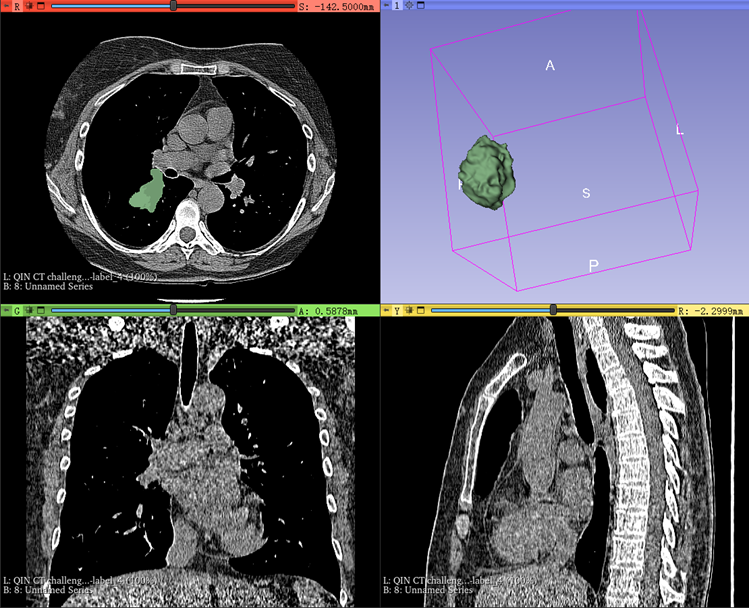
\includegraphics[width=0.7\textwidth]{fig/introduction/3dslicer.png}
    \caption{The model of one \acrshort{ct} set in \acrshort{rider} Lung \acrshort{ct} displayed in 3D Slicer.}
    \label{fig:3dslicer}
\end{figure}

\chapter{Datasets}\label{cpt:dataset}

\section{Dataset Introduction}

For domain adaptation, the variation of preferred modality and scanning protocol should be considered to improve the network's versatility. \acrfull{tcia} \cite{Clark2013} is identified as the primary dataset source for retrieving data for this project to avoid data conflicts. This project selects a subset of the \acrfull{nsclc} dataset \cite{aerts2014decoding}, \acrfull{rider} lung \acrshort{ct} dataset \cite{zhao2015data}, as the source dataset to train the source network, considering its data size and data diversity, Another sub-dataset of \acrshort{nsclc}, \acrshort{nsclc} Radiomics Interobserver1 \cite{wee2019data}, and Lung Tumours dataset from \acrfull{msd} \cite{antonelli2021medical} are selected as the transfer data to finetune the target network.

\subsection{\acrlong{msd}}
 This \acrfull{msd} challenge and dataset aims to provide such resource through the open sourcing of large medical imaging datasets on several highly different tasks, and by standardising the analysis and validation process \cite{antonelli2021medical}. 
 
\subsubsection{Lung Tumours}
The dataset consists of preoperative thin-section \acrshort{ct} scans from
96 patients with non-small cell lung cancer. This data set was selected due to the challenge of segmenting small tumour regions in an image with a large field-of-view \cite{antonelli2021medical}. The dataset consists of training set, testing set, and label set.

\lists{number}{
	\item For training set, it includes 64 \acrshort{ct} \acrshort{nifti} files.
	\item For testing set, it includes 32 \acrshort{ct} \acrshort{nifti} files.
        \item For label set, it includes 64 segmentation \acrshort{nifti} files.
}

\begin{figure}[h]
    \centering
    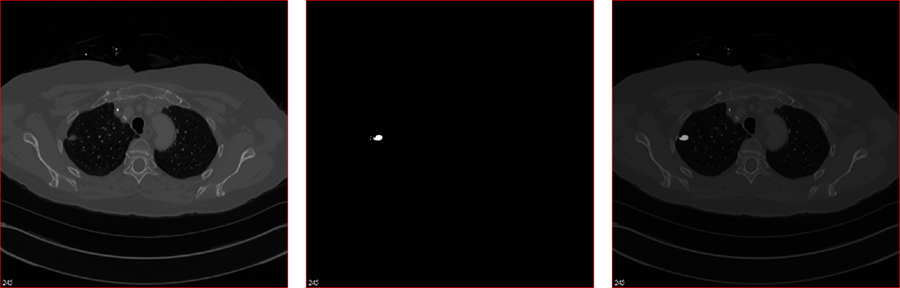
\includegraphics[width=\textwidth]{fig/msd_example.png}
    \caption{The training, label, and composite \acrshort{ct} image of "lung\_001.nii.gz" in \acrshort{msd} lung tumour dataset at frame 245.}
    \label{fig:msd_example}
\end{figure}

\subsection{\acrlong{nsclc}}

The \acrfull{nsclc} dataset is published in Nature Communications which applies a radiomic approach to computed tomography data of 1,019 patients with lung or head-and-neck cancer \cite{aerts2014decoding}. Radiomics refers to the comprehensive quantification of tumour phenotypes by applying a large number of quantitative image features \cite{aerts2014decoding}. This project introduces two lung tumour relevant datasets through manual delineation of the 3D volume of the tumor.

\begin{figure}[h]
    \centering
    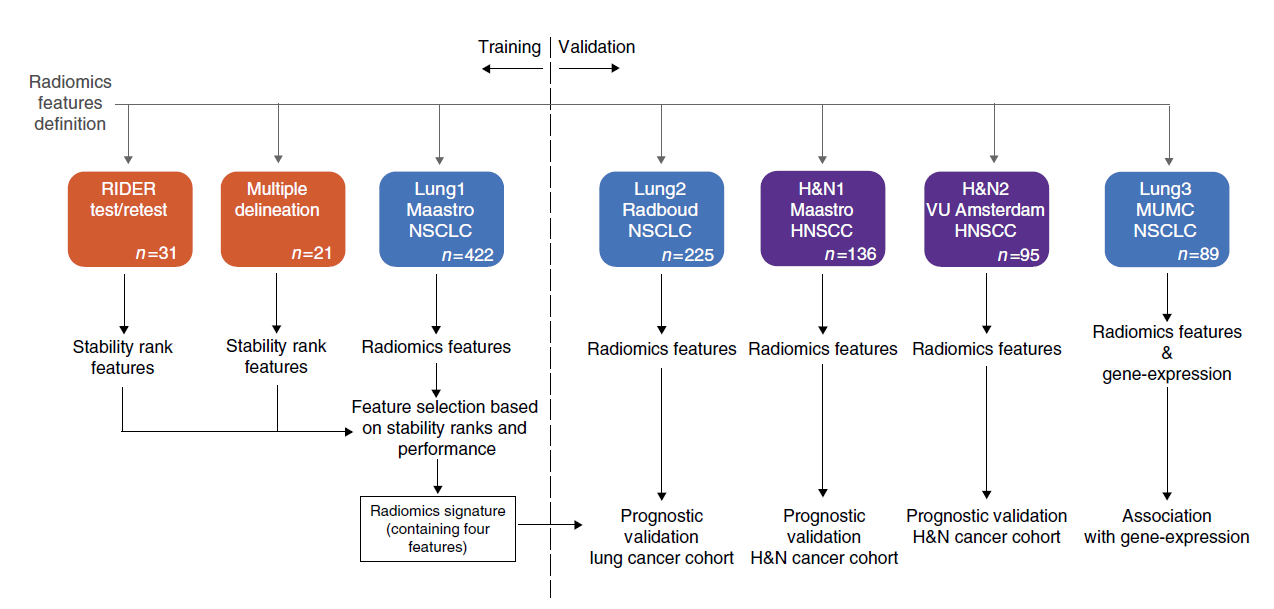
\includegraphics[width=\textwidth]{fig/nsclc_workflow.png}
    \caption{Analysis workflow of this datasets collection which includes \acrshort{rider} datasets and \acrshort{nsclc} Radiomics datasets \cite{aerts2014decoding}.}
    \label{fig:nsclc_workflow}
\end{figure}

\subsubsection{\acrshort{rider} Lung \acrshort{ct}}
\acrfull{rider} Lung \acrshort{ct} collection was constructed as part of a study to evaluate the variability of tumor unidimensional, bidimensional, and volumetric measurements on same-day repeat \acrshort{ct} scans in patients with non–small cell lung cancer \cite{zhao2015data}. The dataset consists of raw resources (\acrshort{rider} Lung \acrshort{ct}) \cite{zhao2015data} and third party analyses (\acrshort{rider}-LungCT-Seg) \cite{wee2020data}.


\lists{number}{
	\item For \acrshort{rider} Lung \acrshort{ct}, it includes 63 \acrshort{ct} DICOM series from 63 patients.
	\item For \acrshort{rider}-LungCT-Seg, it includes 59 relevant SEG and RESTRUCT \acrshort{dicom} series.
}

\begin{figure}[h]
    \centering
    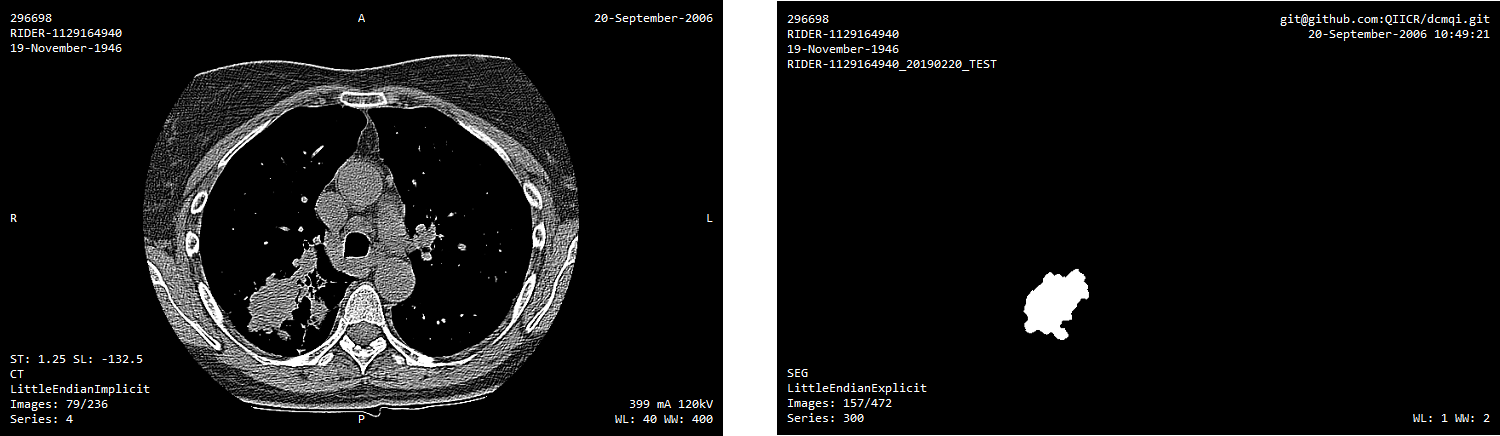
\includegraphics[width=\textwidth]{fig/rider_example2.png}
    \caption{The raw and segmentation \acrshort{ct} image of "RIDER-1129164940" in \acrshort{rider} lung tumour dataset at frame 157.}
    \label{fig:rider_example2}
\end{figure}

\subsubsection{\acrshort{nsclc}-Radiomics-Interobserver1}

This collection contains clinical data and \acrshort{ct} from 22 non-small cell lung cancer radiotherapy patients \cite{wee2019data}. The dataset consists of \acrshort{ct} and segmentation as well.

\lists{number}{
	\item For \acrshort{ct}, it includes 22 \acrshort{ct} \acrshort{dicom} series from 22 patients.
	\item For segmentation, it includes 22 relevant SEG and RESTRUCT \acrshort{dicom} series.
}

\begin{figure}[h]
    \centering
    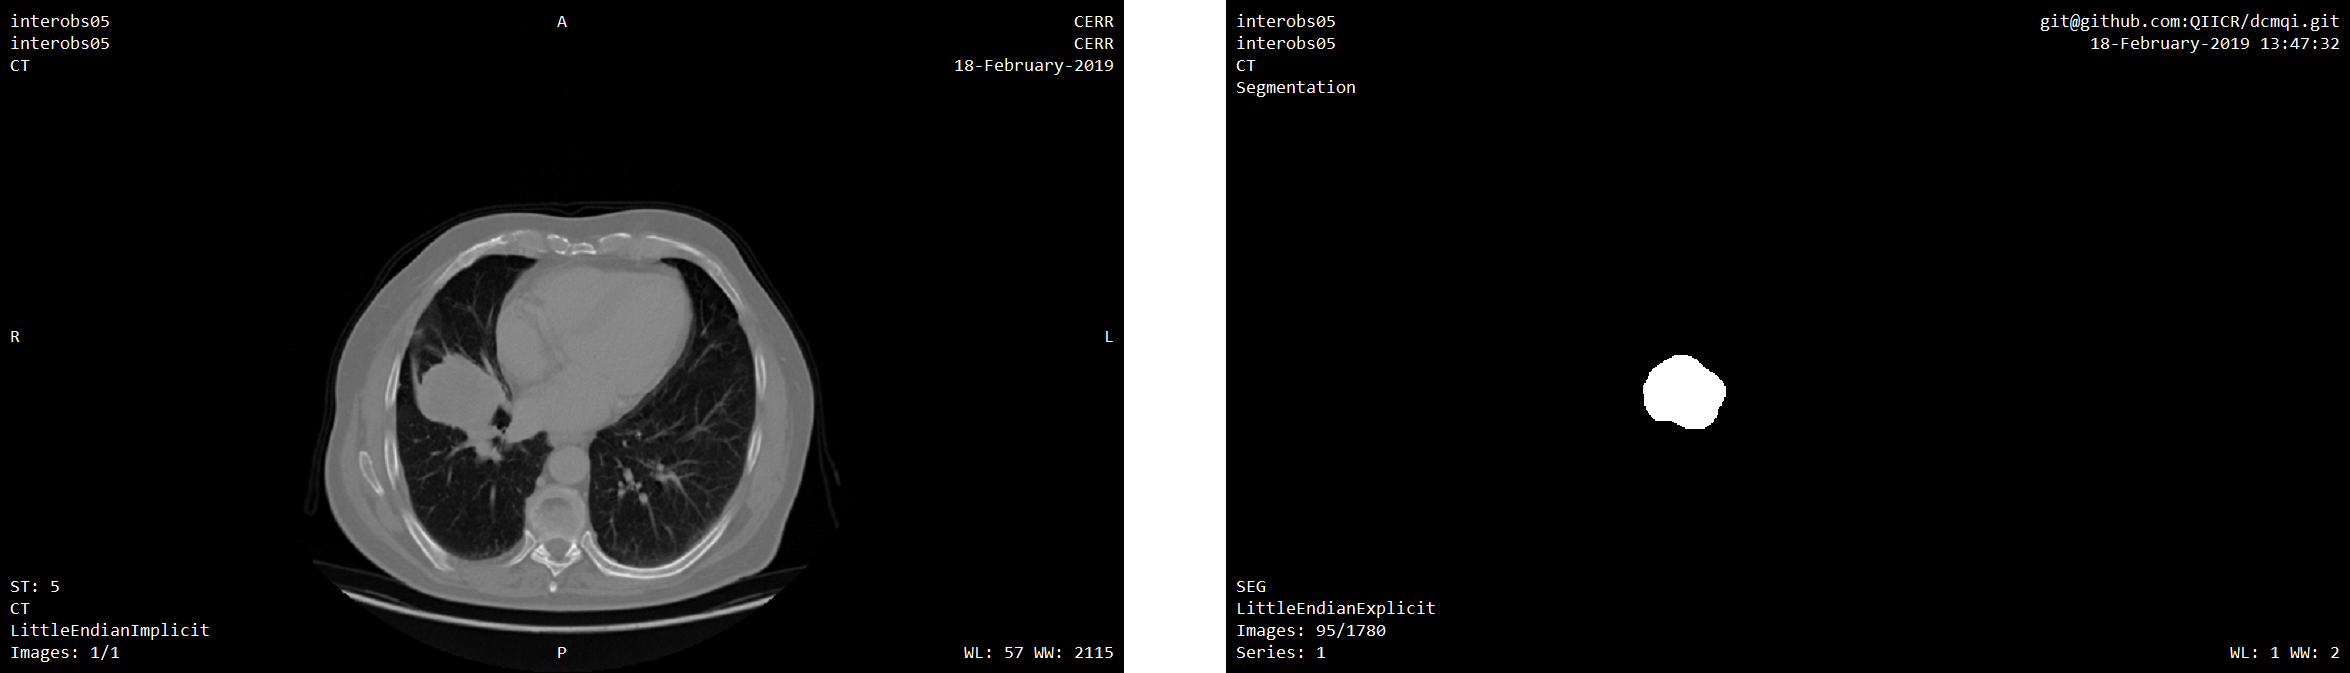
\includegraphics[width=\textwidth]{fig/nsclc_example_dicom.png}
    \caption{The raw and segmentation \acrshort{ct} image of "interobs05" in \acrshort{nsclc} Radiomics Interobserver1 lung tumour dataset at frame 95.}
    \label{fig:nsclc_example_dicom}
\end{figure}

\section{Dataset Format}

\subsection{\acrlong{nifti}}

\acrfull{nifti} is a new Analyze-style data format as a short-term measure to facilitate inter-operation of functional \acrshort{mri} data analysis software packages \cite{jonnalagadda2009nifti}. The original format of \acrshort{msd} datasets is \acrshort{nifti}.

\begin{figure}[h]
    \centering
    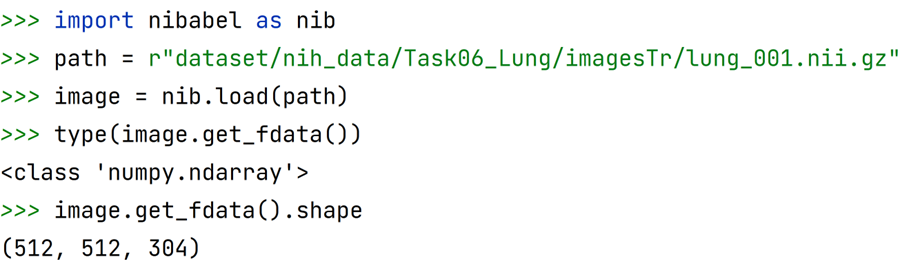
\includegraphics[width=\textwidth]{fig/nii_import.png}
    \caption{The \acrshort{nifti} file loading process of "lung\_001.nii.gz" in \acrshort{msd} lung tumour dataset.}
    \label{fig:nii_import}
\end{figure}

\subsection{\acrlong{dicom}}
\acrfull{dicom} is the international standard for medical images and related information \cite{mustra2008overview}. The raw \acrshort{ct} radiomic images in the \acrshort{nsclc} datasets are all in the \acrshort{dicom} format. \acrfull{dcmqi} is a protocol with minimum dependencies to support standardized communication of quantitative image analysis research data using \acrshort{dicom} standard \cite{herz2017dcmqi}. The segmentation slices in the \acrshort{nsclc} datasets are all in the \acrshort{dcmqi} format.

\subsection{Medical Format Normalization}
Considering the less metadata and better performance in 3D volumn representation, this project prefers to use \acrshort{nifti} as an intermediate format towards NumPy array. NumPy arrays as a standard matrix format provide more transformation functions and better compatibility with PyTorch. The specific reformatting path is depicted in the Fig \ref{fig:reformat_path}, where some third-party tools are introduced, such as dcm2niix and dcmqi.

\begin{figure}[h]
    \centering
    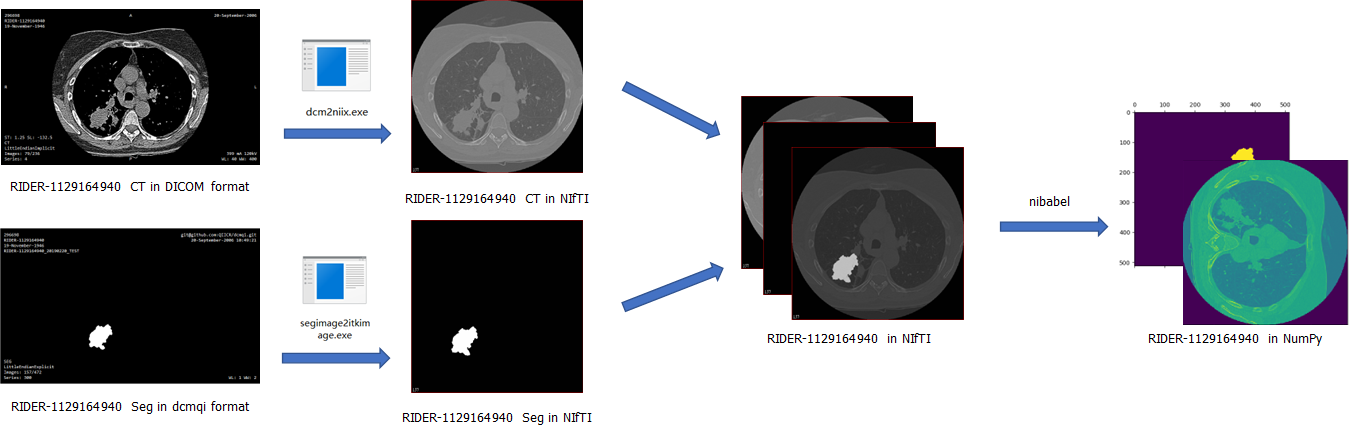
\includegraphics[width=\textwidth]{fig/reformat_path.png}
    \caption{The files reformating process from \acrshort{dicom} and \acrshort{dcmqi} to \acrshort{nifti} and finally NumPy arrays.}
    \label{fig:reformat_path}
\end{figure}

\section{Dataset Preprocess}
\subsection{Resampling}
Due to the different voxel coordinates of \acrshort{ct} and segmentation series, the \acrshort{ct} and segmentation volumes are resampled to the unit voxel size of \(1mm\times1mm\times1mm\). The resampling transformation is applied by matrix multiplication with the affine matrix, which is defined as
\begin{equation}
\left[\begin{array}{c}
x \\
y \\
z \\
1
\end{array}\right]=\left[\begin{array}{cccc}
m_{1,1} & m_{1,2} & m_{1,3} & a \\
m_{2,1} & m_{2,2} & m_{2,3} & b \\
m_{3,1} & m_{3,2} & m_{3,3} & c \\
0 & 0 & 0 & 1
\end{array}\right]\left[\begin{array}{c}
i \\
j \\
k \\
1
\end{array}\right]
\end{equation}
\subsection{Cube Bounding}
Cube bounding is utilized to crop the \acrshort{ct} and segmentation volumes to emphasize the tumour area and reduce unwanted background. The cube box is centered on the center of the tumour volumes, with enough side length and fixed pads to cover the whole target volumes and necessary backgrounds.
\begin{figure}[h]
    \centering
    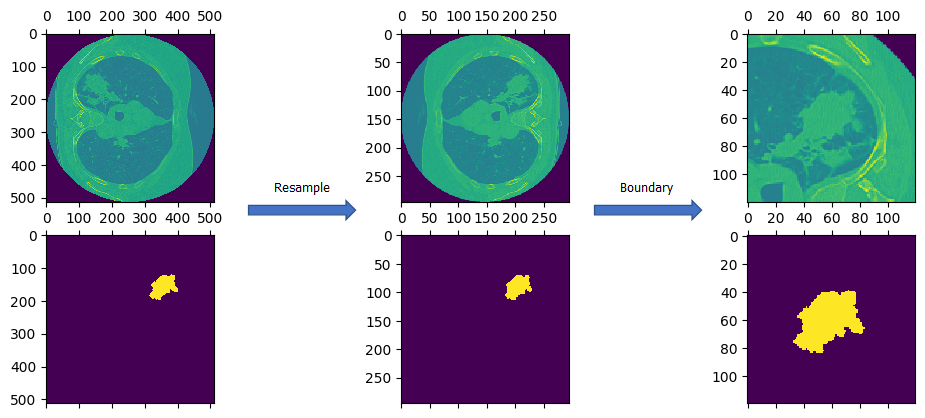
\includegraphics[width=\textwidth]{fig/preprocess_path.png}
    \caption{The data preprocessing process through resampling and cube bounding.}
    \label{fig:preprocess_path}
\end{figure}

\section{Data Augmentation}
Data augmentation is often used to handle the problem of the data shortage and insufficient training samples, especially for 3D segmented medical images. In model fitting, it can alleviate the overfitting problem for models with strong generalization capabilities and robustness \cite{taylor2018improving}. This project applies geometric methods for this process, including scaling, rotation and cropping in a random range. The volumes are through normalization mapped to \(\left [ 0, 1 \right ]\) at beginning and centered in the patch volumes in the end to standardize the volume size and range.

\begin{figure}[h]
    \centering
    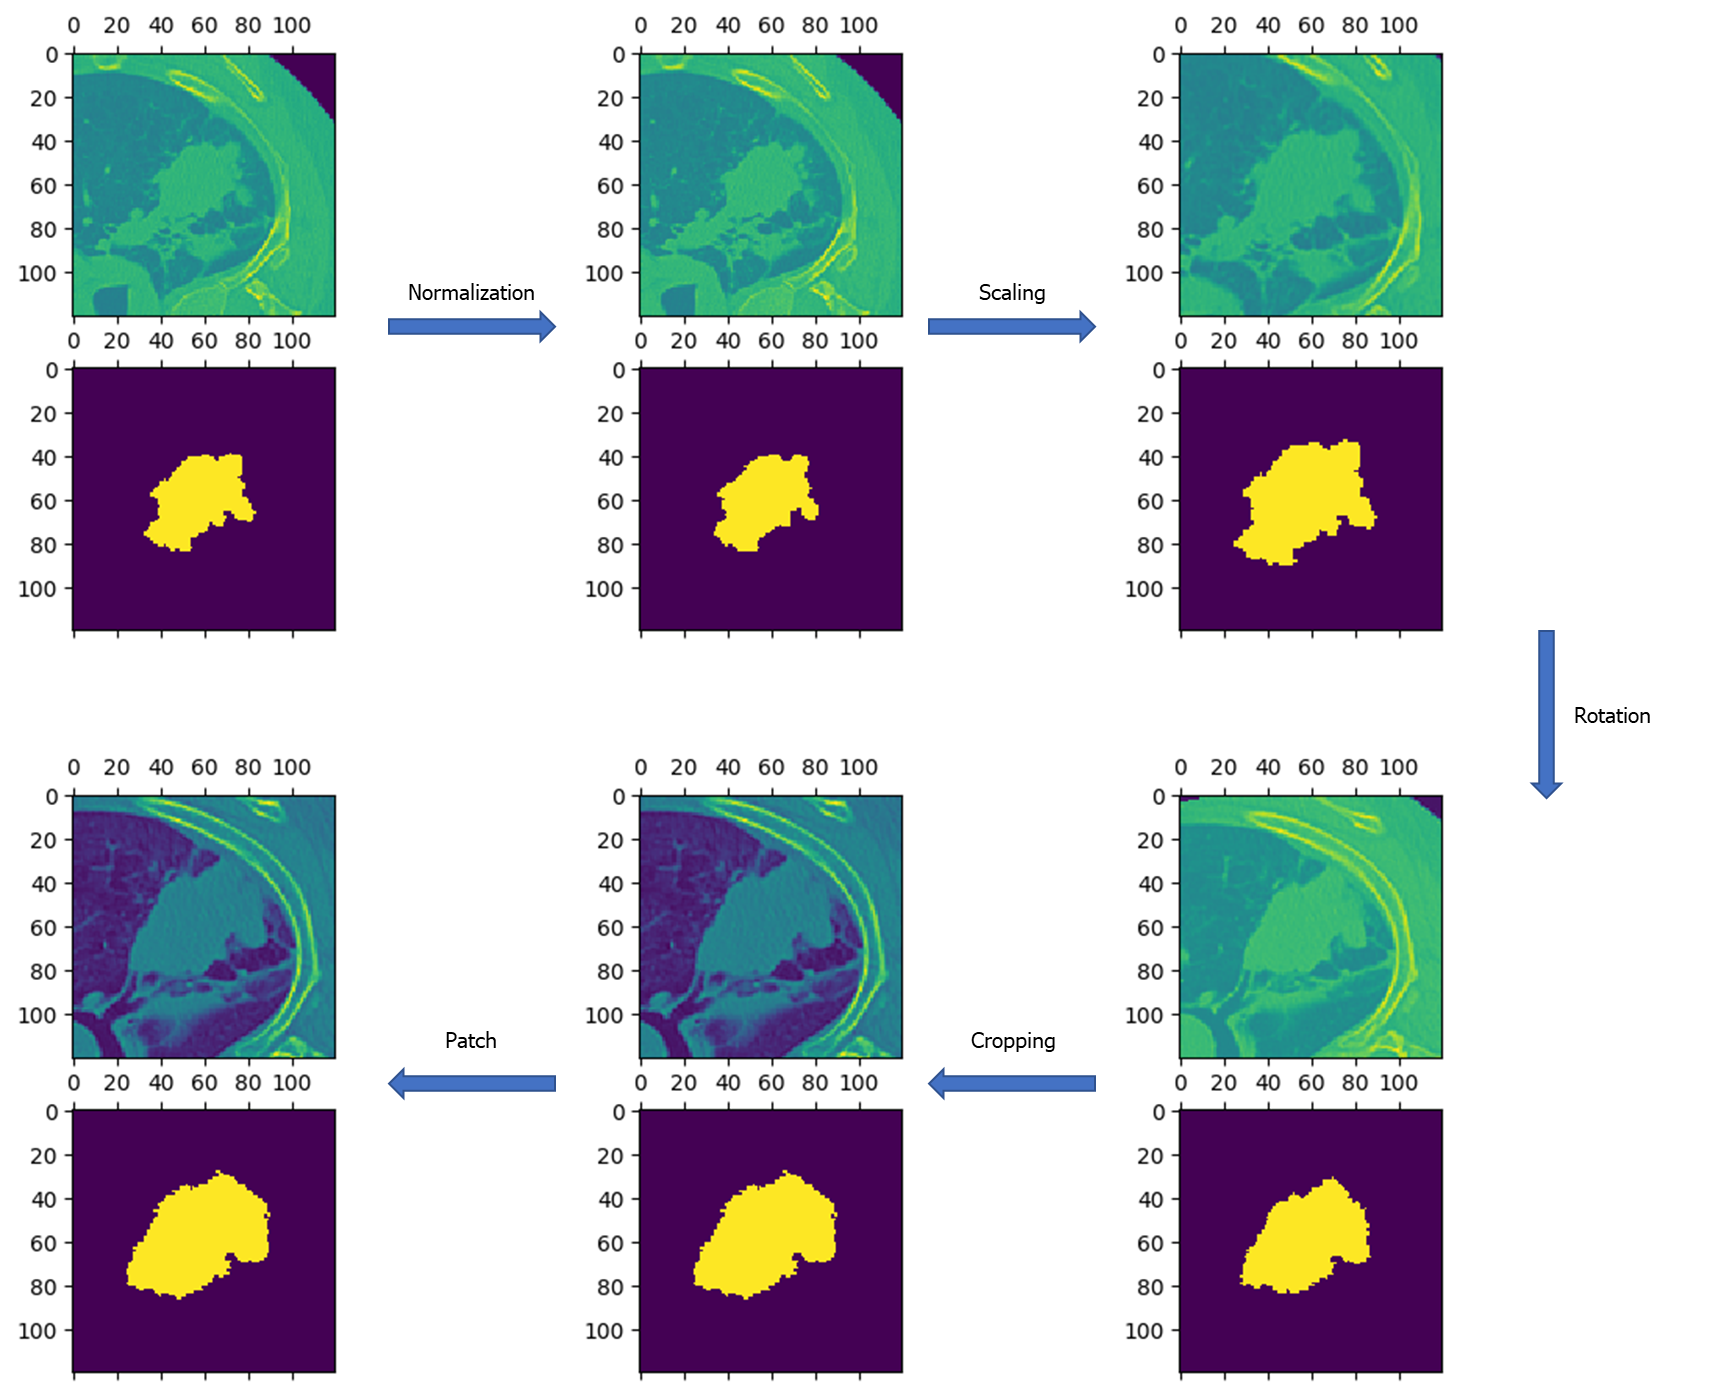
\includegraphics[width=\textwidth]{fig/dataset/augmentation.png}
    \caption{The data augmentation process through normalization, scaling, rotation, cropping and patch.}
    \label{fig:augmentation}
\end{figure}

\chapter{Methodology}\label{cpt:method}

\section{Method Background}

\subsection{3D \acrlong{cnn}}
\acrfull{cnn} is a neural network primarily applied
on images. 3D \acrshort{cnn} is constructed by convolutional layers convolving 3D kernels to the cube formed by stacking multiple-dimensional spatial features, compared with 2D \acrshort{cnn}, where convolutions are applied on the 2D feature maps to compute features from the single layers only \cite{ji20123d}. According to \citet{ji20123d}, the formula of the value at position \((x, y, z)\) on the $j$th feature map in the $i$th layer is given by
\begin{equation}
v_{i j}^{x y z}=\tanh \left(b_{i j}+\sum_{m} \sum_{p=0}^{P_{i}-1} \sum_{q=0}^{Q_{i}-1} \sum_{r=0}^{R_{i}-1} w_{i j m}^{p q r} v_{(i-1) m}^{(x+p)(y+q)(z+r)}\right) \text {, }
\end{equation}
where \((P_{i}, Q_{i}, R_{i})\) is the size of the 3D kernel, and \(w^{pqr}_{ijm}\) is the ($p$, $q$, $r$)th value of the kernel connected to the $m$th feature map in the previous layer.

\begin{figure}[h]
    \centering
    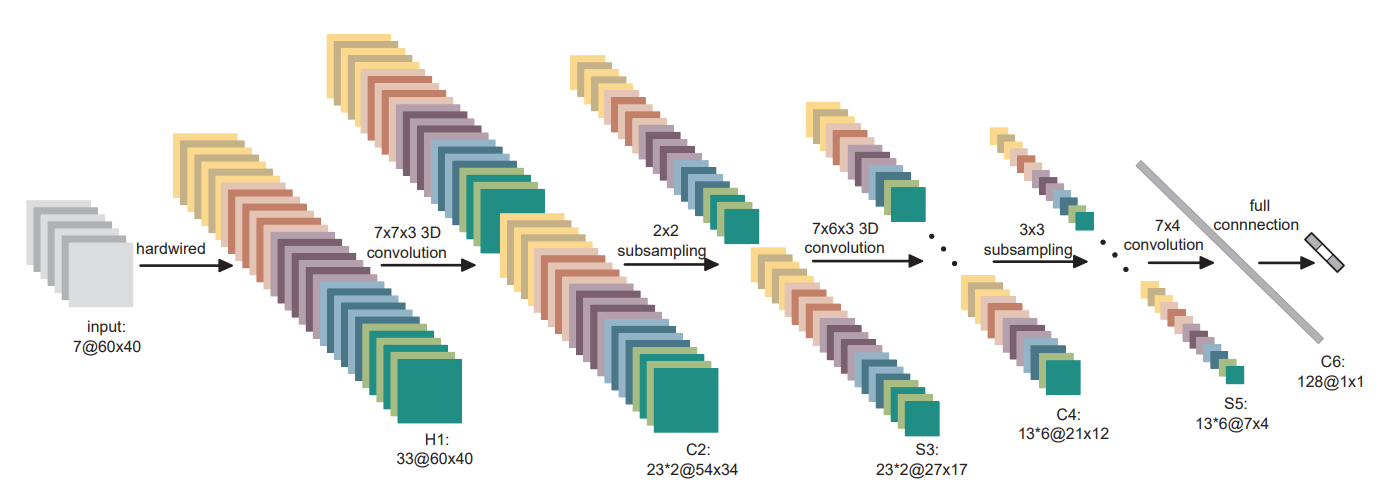
\includegraphics[width=\textwidth]{fig/methodology/3dcnn.png}
    \caption{An example 3D \acrshort{cnn} architecture for human action recognition \citet{ji20123d}.}
    \label{fig:3dcnn}
\end{figure}

In this project, 3D \acrshort{cnn} serves as the basic network block for feature extraction. With relevant deconvolutional networks, segmentation mask can be constructed in image segmentation task. 

\subsection{\acrlong{vit}}

Self-attention-based architectures, such as Transformers, have been widely used in the field of \acrfull{nlp}. In image recogniztion, \citet{dosovitskiy2020image} introduce \acrfull{vit} architecture which abandons the traditional \acrshort{cnn} structure and applies a standard Transformer directly to images. The images are divided into patches linked with the linear sequence, which are seen as tokens in term of \acrshort{nlp} \cite{dosovitskiy2020image}. 

\begin{figure}[h]
    \centering
    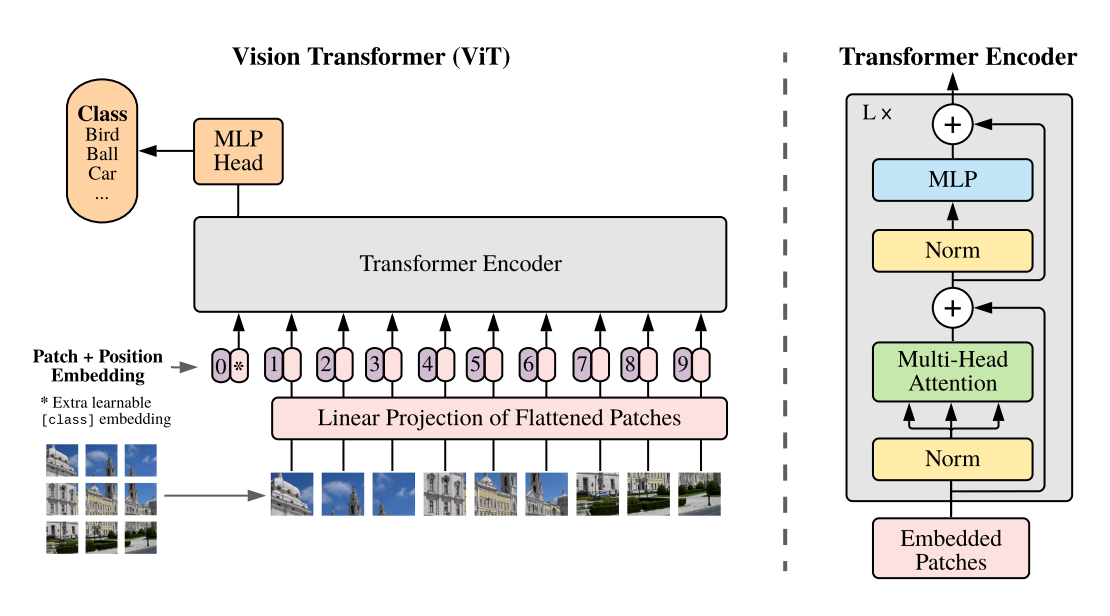
\includegraphics[width=\textwidth]{fig/methodology/vision_transformer.png}
    \caption{The \acrlong{vit} architecture \cite{dosovitskiy2020image}.}
    \label{fig:vision_transformer}
\end{figure}

One transformer encoder process can be defined as

\begin{equation}
    \begin{aligned}
\mathbf{z}_{0} & =\left[\mathbf{x}_{\text {class }} ; \mathbf{x}_{p}^{1} \mathbf{E} ; \mathbf{x}_{p}^{2} \mathbf{E} ; \cdots ; \mathbf{x}_{p}^{N} \mathbf{E}\right]+\mathbf{E}_{p o s}, & & \mathbf{E} \in \mathbb{R}^{\left(P^{2} \cdot C\right) \times D}, \mathbf{E}_{p o s} \in \mathbb{R}^{(N+1) \times D} \\
\mathbf{z}_{\ell}^{\prime} & =\operatorname{MSA}\left(\mathrm{LN}\left(\mathbf{z}_{\ell-1}\right)\right)+\mathbf{z}_{\ell-1}, & & \ell=1 \ldots L \\
\mathbf{z}_{\ell} & =\operatorname{MLP}\left(\mathrm{LN}\left(\mathbf{z}_{\ell}^{\prime}\right)\right)+\mathbf{z}_{\ell}^{\prime}, & & \ell=1 \ldots L \\
\mathbf{y} & =\operatorname{LN}\left(\mathbf{z}_{L}^{0}\right) & &
\end{aligned}
\end{equation}

where MLP is the multilayer perceptron block, \acrshort{msa} is the \acrlong{msa} block, and Layernorm (LN) and residual connection are applied between each network blocks \cite{dosovitskiy2020image}.

\acrfull{msa} is an extension of standard $QKV$ self-attention with $k$ paralleled self-attention operations \cite{dosovitskiy2020image}. The \acrshort{msa} block process can be defined as

\begin{equation}
    \begin{array}{rlrl}
    {[\mathbf{q}, \mathbf{k}, \mathbf{v}]} & =\mathbf{z} \mathbf{U}_{q k v} && \mathbf{U}_{q k v} \in \mathbb{R}^{D \times 3 D_{h}} \\
    A & =\operatorname{softmax}\left(\mathbf{q k}^{\top} / \sqrt{D_{h}}\right) && A \in \mathbb{R}^{N \times N} \\
    \mathrm{SA}(\mathbf{z}) & =A \mathbf{v} \\
    \operatorname{MSA}(\mathbf{z}) &=\left[\mathrm{SA}_{1}(z) ; \mathrm{SA}_{2}(z) ; \cdots ; \mathrm{SA}_{k}(z)\right] \mathbf{U}_{m s a} &&\mathbf{U}_{m s a} \in \mathbb{R}^{k \cdot D_{h} \times D}
    \end{array}
\end{equation}

where $q$, $k$, $v$ are query, key and value matrix \cite{dosovitskiy2020image}.

Althrough transformers lack some of the inductive biases inherent to \acrshort{cnn}s leading to its poor generalization performance on insufficient amounts of data, some researches, such as \acrfull{unetr} \cite{hatamizadeh2022unetr} and TransUNet \cite{chen2021transunet}, show reasonable segmentation scores by combination of \acrshort{cnn}s and transformers \cite{dosovitskiy2020image}.


\section{Main Framework}

\subsection{\acrshort{vae} Pipeline}
\citet{yao2022unsupervised} developed an \acrfull{uda} framework to import inherent shape statistics into a standard medical image segmentation model, which is based on a teacher-student learning paradigm with a dual-loss function.

\begin{figure}[h]
    \centering
    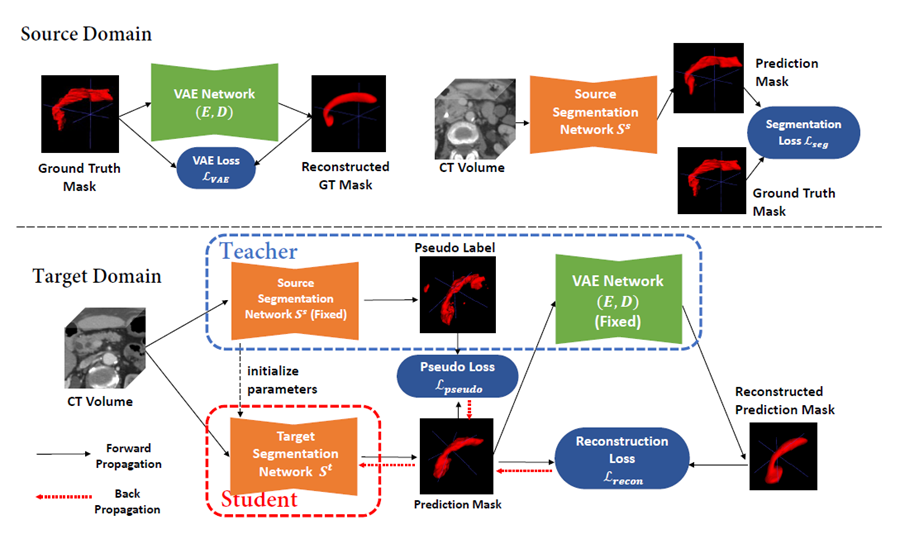
\includegraphics[width=\textwidth]{fig/vae_seg.png}
    \caption{Proposed \acrshort{vae}-based pipeline of \acrlong{uda} \cite{yao2022unsupervised}.}
    \label{fig:vae_seg}
\end{figure}

On the source domain, the organ shape information is extracted through a pre-trained \acrshort{vae} network in ground truth masks \cite{yao2022unsupervised}. One dataset is under the training of source segmentation network (3D \acrshort{unet} in this project) to initialise it as a teacher network. On the target domain, the two trained networks, i.e., the \acrshort{vae} network and source segmentation network, are fixed as teacher networks \cite{yao2022unsupervised}. The target segmentation network is initialised by the source one and loads another unlabeled dataset in a different style from the first dataset for domain adaptation \cite{yao2022unsupervised}. The pseudo label is generated by the source segmentation network in the teacher group for a pseudo-loss calculation to fine-tune the segmentation labels \cite{yao2022unsupervised}. The distribution of shape for a specific organ is from the \acrshort{vae} network in the teacher group to predict reconstructed masks and acquire reconstruction loss \cite{yao2022unsupervised}. The dual loss is combined by a loss function with a hyperparameter offset \(\lambda\), defined in Equation \ref{eq:dual_loss}, considering their adverse effects \cite{yao2022unsupervised}.

\begin{equation} \label{eq:dual_loss}
    L_{\theta}\left(S^{t}, x^{t}\right)=\lambda_{\text {recon }} \cdot \mathcal{L}_{\text {recon }}+\mathcal{L}_{\text {pseudo }}
\end{equation}

\section{Segmentation Network}

\subsection{3D \acrshort{unet}}

3D \acrshort{unet} is a \acrshort{cnn}-based network for image segmentation which learns from sparsely annotated volumetric images \cite{cciccek20163d}. The network extends the previous \acrshort{unet} architecture from \citet{ronneberger2015u} by replacing all 2D operations in dimensions with 3D counterparts \cite{cciccek20163d}. Similar to the standard \acrshort{unet}, this network contains two paths, including an analysis one and a synthesis one, each with four resolution layers, depicted in Fig \ref{fig:3dunet} \cite{cciccek20163d}.

\begin{figure}[h]
    \centering
    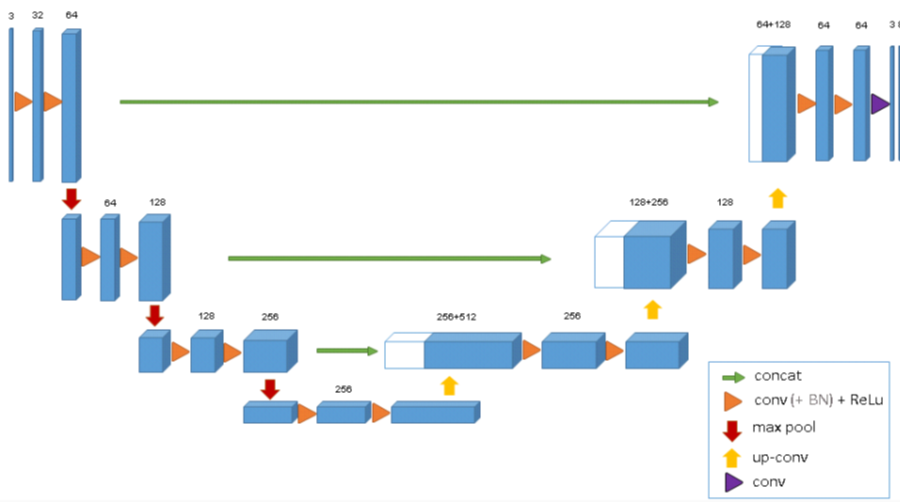
\includegraphics[width=\textwidth]{fig/3dunet.png}
    \caption{The 3D \acrshort{unet} network architecture \cite{cciccek20163d}.}
    \label{fig:3dunet}
\end{figure}

This means one medical image can be labelled in the target domains to realise semantic segmentation. In this project, the framework is modified to fit the dataset magnitude.
\lists{number}{
	\item In the analysis path, all four "Down" layers contain one \(2\times2\times2\) convolution layer alone with a stride of two in all dimensions, and three same convolution layers each followed by an activation function (ReLu or Softplus) and a normalisation layer (Instance Normalisation or Batch Normalisation). The max pooling layer in the original 3D \acrshort{unet} model is not applied, which is replaced by an optional dropout layer. 
	\item In the synthesis path, all four "Up" layers consist of the up-convolution layers whose structure and parameters are similar to the "Down" ones but in the opposite direction.
	\item Shortcut connections from layers of equal resolution between analysis and synthesis paths remain to import high-resolution features realised by concatenation.
	\item In the last layer, a convolution layer reduces the number of output channels to the number of labels. Then, a Softmax function is attached to get the final labels for each point.
}

\subsection{\acrlong{unetr}}

\acrfull{unetr} follows 3D \acrshort{unet} “U-shaped” network design for the encoder and decoder, but replaces the CNN layers with a \acrshort{vit} transformer in the encoder to consider volume sequence representations and capture the multi-dimension information \cite{hatamizadeh2022unetr}.

\begin{figure}[h]
    \centering
    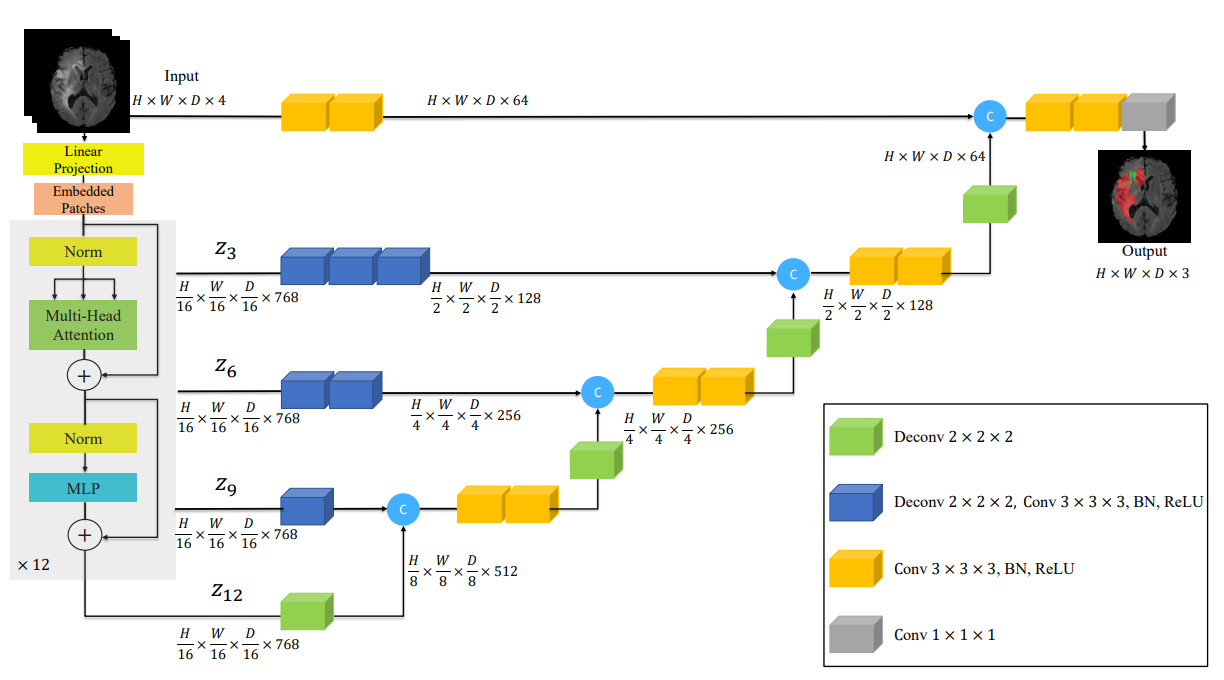
\includegraphics[width=\textwidth]{fig/unetr.png}
    \caption{The \acrshort{unetr} network architecture \cite{hatamizadeh2022unetr}.}
    \label{fig:unetr}
\end{figure}

According to \acrshort{vit}, a 1D sequence of a 3D input volume is initialized by splitting it into flattened patches and embeded with its positional sequence at beginning \cite{hatamizadeh2022unetr}. In encoder path, the twelve transformer blocks are divided into four stack of transformers, which can be seen as encoder layers \cite{hatamizadeh2022unetr}. Similar to 3D \acrshort{unet}, features from multiple resolutions of the encoder are merged with the decoder by concatenating volumes in the same level \cite{hatamizadeh2022unetr}. However, the hidden layer outputs need to reshaped into the target volume size and encoded through some deconvolution blocks \cite{hatamizadeh2022unetr}. Compared with standard 3D \acrshort{unet}, \acrshort{unetr} discards max-pooling layers between levels, which increases the parameter size.

\section{Model Shaping Network}

\subsection{\acrlong{vae}}

The \acrfull{vae} is applied for the recognition, denoising, representation and visualisation by learning the approximate posterior inference model \cite{kingma2013auto}. The \acrshort{vae} network consists of Encoder and Decoder at the architecture level \cite{kingma2013auto}. To allow back propagation, the reparameterisation trick is introduced in the sampling function, which combines the distribution parameters (mean and standard deviation) and a random sampled number in a scale \cite{kingma2013auto}. Through \acrshort{kl} divergence, Gaussian distribution, and Bayes formula, the final result formula of the \acrshort{vae} can be presented as the one in Equation \ref{eq:vae}, under the reparameterisation trick \cite{kingma2013auto}. This means one image can be sampled into features as a latent variable and re-sampled to restore the original image.

\begin{equation} \label{eq:vae}
    \begin{aligned}
    \mathcal{L}\left(\theta, \phi ; x^{(i)}\right) \simeq & \frac{1}{2} \sum_{j=1}^{J}\left(1+\log \left(\left(\sigma_{j}^{(i)}\right)^{2}\right)-\left(\mu_{j}^{(i)}\right)^{2}-\left(\sigma_{j}^{(i)}\right)^{2}\right) \\
    & +\frac{1}{L} \sum_{l=1}^{L} \log p_{\theta}\left(x^{(i)} \mid \mathbf{z}^{(i, l)}\right) \\
    \text { where } \mathbf{z}^{(i, l)}= & \mu^{(i)}+\sigma^{(i)} \odot \epsilon^{(l)} \text { and } \epsilon^{(l)} \sim \mathcal{N}(0, \mathbf{I})
    \end{aligned}
\end{equation}

In this project, the reconstructed mask, i.e., the shape information of labels, must be extracted by the \acrshort{vae} network trained with ground truth masks. The structure follows the original design of the \acrshort{vae} network but imports the Dice coefficient as the loss term.
\lists{number}{
        \item In the encoder block, all five encoding layers contain one \(2\times2\times2\) convolution layer alone and three same convolution layers, followed by an activation function and a normalisation layer. The encoding layers and their parameters are analogous to the "Down" layer in the 3D \acrshort{unet}, which reuse the layer-building function.
	\item In the decode block, all five decoding layers consist of the up-convolution layers whose structure and parameters are similar to the encoding ones but in the opposite direction, which is analogous to the "Up" layer.
	\item The mean and standard deviation are calculated in the middle layers for back propagation. For the reparameterisation trick, the random sample between zero and a given scale is optional.
	\item In the last layer, a convolution layer reduces the number of output channels to the number of labels. Then, a Softmax function is attached to get the final labels for each point.
}

\begin{figure}[h]
    \centering
    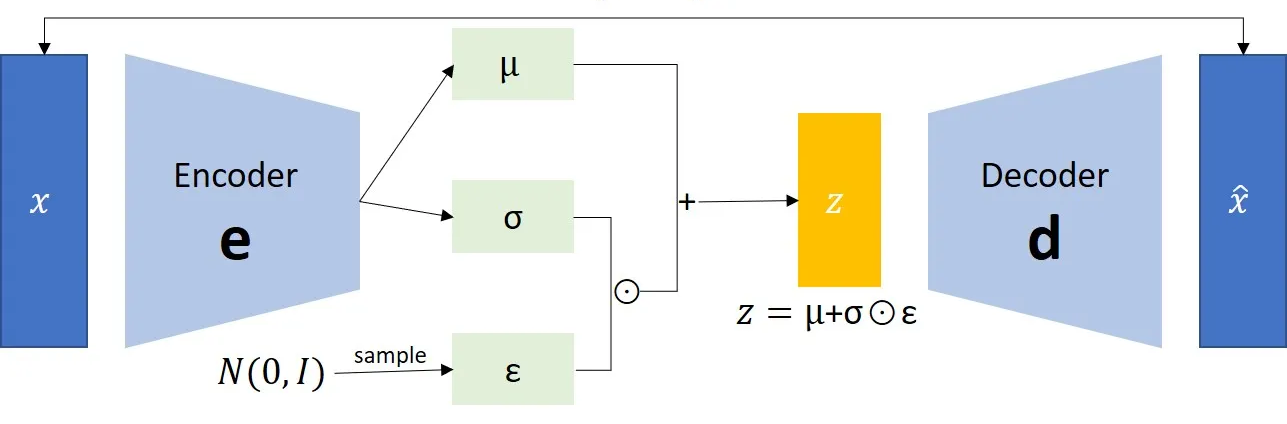
\includegraphics[width=\textwidth]{fig/vae.png}
    \caption{The \acrshort{vae} architecture \cite{kingma2013auto}.}
    \label{fig:vae}
\end{figure}

% \subsection{Generative Adversarial Networks}

% \begin{figure}[h]
%     \centering
%     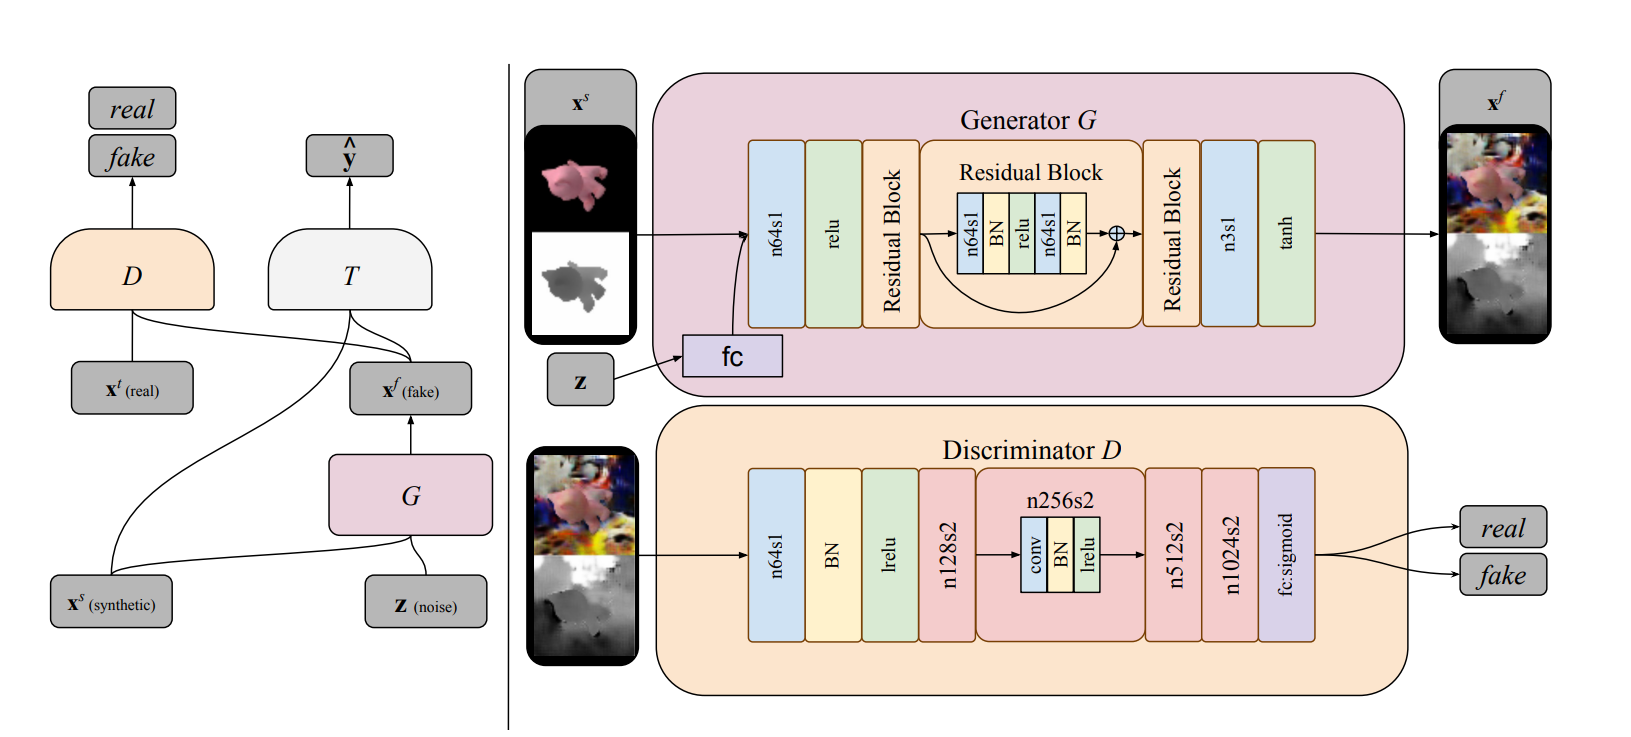
\includegraphics[width=\textwidth]{fig/methodology/gan.png}
%     \caption{The architecture of variational autoencoder.}
%     \label{fig:gan}
% \end{figure}

\section{Loss Function}
Tumour areas in this lung tumour segmentation task represent a very small fraction of the full image in some slices. Such unbalanced problems can cause improper fitting such as a tendency to mark all to non-tumour leading to false negative results, applying inappropriate loss functions \cite{sudre2017generalised}. This project prefers to apply the Dice loss for evaluation and validation.
\subsection{Dice Loss}
The Dice score coefficient is a measure of overlap widely
used to assess segmentation performance when ground truth is available. The Dice loss can be expressed as

\begin{equation}
    DL_{s}=1-\frac{2|X \bigcap Y| + \epsilon }{|X|+|Y| + \epsilon}
\end{equation}
where \(|X \bigcap Y|\) is the intersection between X and Y, \(|X|\) and \(|Y|\) are the numbers of elements of X and Y, and\(\epsilon\) is the smoothing parameter for Laplace smoothing \cite{sudre2017generalised}.

Multiple labels Dice loss for Tensor is implemented, as it is not realized in PyTorch.

\lstinputlisting[language=Python]{code/dice_loss.py}

\chapter{Experiments}

\section{Experiment Process}

\subsection{Train on source domain}
Three datasets (\acrshort{msd}, \acrshort{rider}, and \acrshort{nsclc}) have been trained on the two segmentation models (3D \acrshort{unet} and \acrshort{unetr}) and shaping model (\acrshort{vae}) respectively with relevant labelled segmentaion masks to access the upper bound scores. The pre-trained models are saved for best model selection and further domain adaptation in target domain.
\subsection{Train on target domain}
The pre-trained segmentation and shaping models of one dataset are selected as the source dataset to initialize parameters in the two fixed teacher networks. The other two datasets left are target datasets to fine-tune the student segmentation network, where their ground truth masks are neglected as they are in unsupervised domain adaptation. The three datasets are determined to be the source dataset to observe their performance.

\section{Results}

% {
% \centering
% \begin{tabular}{ |>{\centering\arraybackslash}m{3cm}||>{\centering\arraybackslash}m{3cm}|>{\centering\arraybackslash}m{3cm}|>{\centering\arraybackslash}m{3cm}|  }
%  \hline
%   &MSD\cite{zhao2015data}&RIDER\cite{wee2019data}&NSCLC-1\cite{wee2020data}\\
%  \hline
%  Direct&\slash&0.6637&0.6928\\
%  UDA&\slash&0.6707&0.6956\\
%  Upper Bound&0.7702&0.7241&0.6706\\
%  \hline
% \end{tabular}\par
% }
\subsection{Model Performance}
Table \ref{tab:3dunet_result} and Table \ref{tab:unetr_result} present the segmentation results on 3D \acrshort{unet} and \acrshort{unetr} as their segmentation models, which are evaluated with mean Dice score. In detail, the data in columns have same target datasets. The upper bound score means the result in the segmentation model trained by relevant labelled datasets, which can be seen as ceiling score. The direct score means validate the dataset on the model trained by another dataset without any finetune. The \acrshort{uda} score is the final score through the complete model. Domain adaptation do polish up the score from direct validation. Moreover, due to more fitting on a larger dataset, the \acrshort{uda} even have better score on the small \acrshort{nsclc} dataset.
{
\centering
\begin{table}[]
\begin{tabularx}{\textwidth}{|>{\centering\arraybackslash}X>{\centering\arraybackslash}X||>{\centering\arraybackslash}X|>{\centering\arraybackslash}X|>{\centering\arraybackslash}X|}
\hline
\multicolumn{2}{|c||}{}                                & \acrshort{msd}    & \acrshort{rider}  & \acrshort{nsclc}  \\ \hline
\multicolumn{2}{|c||}{Upper Bound}                     & 0.6676 & 0.7879 & 0.6963 \\ \hline
\multicolumn{1}{|c|}{\multirow{3}{*}{Direct}} & \acrshort{msd}   & /      & 0.7247 & 0.7248 \\ 
\multicolumn{1}{|c|}{}                        & \acrshort{rider} & 0.6537 & /      & 0.7511 \\ 
\multicolumn{1}{|c|}{}                        & \acrshort{nsclc} & 0.6065 & 0.6382 & /      \\ \hline
\multicolumn{1}{|c|}{\multirow{3}{*}{\acrshort{uda}}}    & \acrshort{msd}   & /      & \textbf{0.7415} & 0.7145 \\ 
\multicolumn{1}{|c|}{}                        & \acrshort{rider} & \textbf{0.6625} & /      & \textbf{0.7637} \\ 
\multicolumn{1}{|c|}{}                        & \acrshort{nsclc} & 0.6065 & 0.6669 & /      \\ \hline
\end{tabularx}
\caption{\label{tab:3dunet_result}Performance of this UDA segmentation method
on 3D U-Net.}
\end{table}
}

{
\centering
\begin{table}[]
\begin{tabularx}{\textwidth}{|>{\centering\arraybackslash}X>{\centering\arraybackslash}X||>{\centering\arraybackslash}X|>{\centering\arraybackslash}X|>{\centering\arraybackslash}X|}
\hline
\multicolumn{2}{|c||}{}                                & \acrshort{msd}    & \acrshort{rider}  & \acrshort{nsclc}  \\ \hline
\multicolumn{2}{|c||}{Upper Bound}                     & 0.6708 & 0.7568 & 0.7020 \\ \hline
\multicolumn{1}{|c|}{\multirow{3}{*}{Direct}} & \acrshort{msd}   & /      & 0.6811 & 0.7265 \\ 
\multicolumn{1}{|c|}{}                        & \acrshort{rider} & 0.6547 & /      & 0.7424 \\ 
\multicolumn{1}{|c|}{}                        & \acrshort{nsclc} & 0.5994 & 0.6192 & /      \\ \hline
\multicolumn{1}{|c|}{\multirow{3}{*}{\acrshort{uda}}}    & \acrshort{msd}   & /      & \textbf{0.7326} & 0.7386 \\ 
\multicolumn{1}{|c|}{}                        & \acrshort{rider} & \textbf{0.6624} & /      & \textbf{0.7432} \\ 
\multicolumn{1}{|c|}{}                        & \acrshort{nsclc} & 0.6041 & 0.6357 & /      \\ \hline
\end{tabularx}
\caption{\label{tab:unetr_result}Performance of this UDA segmentation method
on UNETR.}
\end{table}
}

\subsection{Training Process}
Data visualization on training process of validation score is shown in the Fig \ref{fig:unetr_val}, Fig \ref{fig:vae_val}, and Fig \ref{fig:unetr_uda_val}, which are based on \acrshort{unetr} model. As the figures show, the models in source domain can converge quickly in 20 epochs and be stabilised to a upper limit with some fluctuations. The target domain do not provide reasonable finetune towards target datasets. All charts including training losses and validation scores on 3D \acrshort{unet} and \acrshort{unetr} are listed in the Appendix \ref{appendix:charts}. 

\begin{figure}[h]
    \centering
    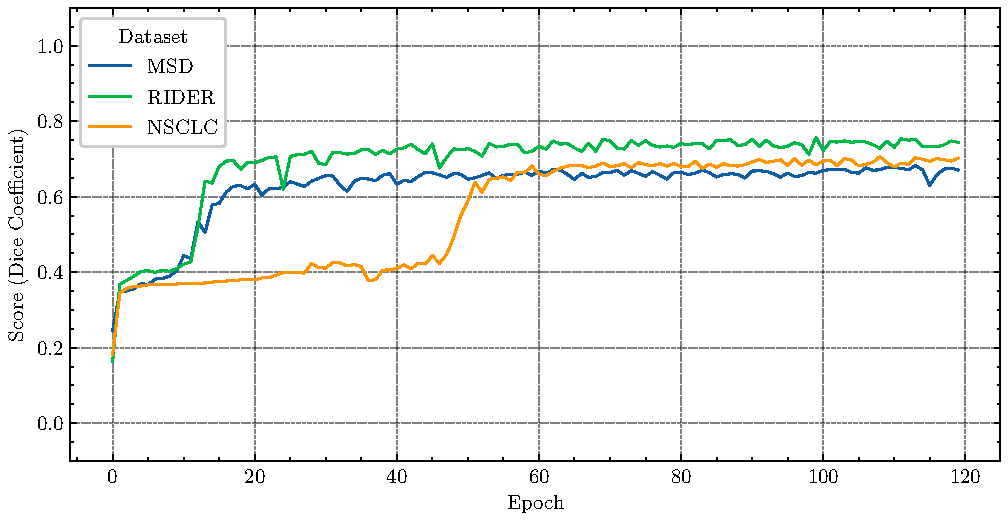
\includegraphics[width=0.95\textwidth]{fig/result/unetr_val.pdf}
    \caption{The validation score chart for three datasets in \acrshort{unetr} segmentation model.}
    \label{fig:unetr_val}
\end{figure}

\begin{figure}[h]
    \centering
    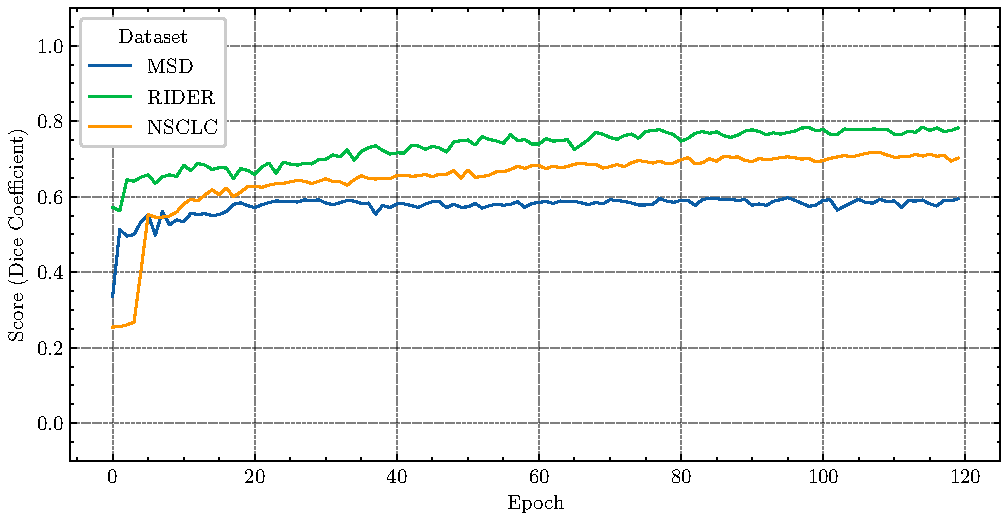
\includegraphics[width=0.95\textwidth]{fig/result/vae_val.pdf}
    \caption{The validation score chart for three datasets in \acrshort{vae} shaping model.}
    \label{fig:vae_val}
\end{figure}

\begin{figure}[h]
    \centering
    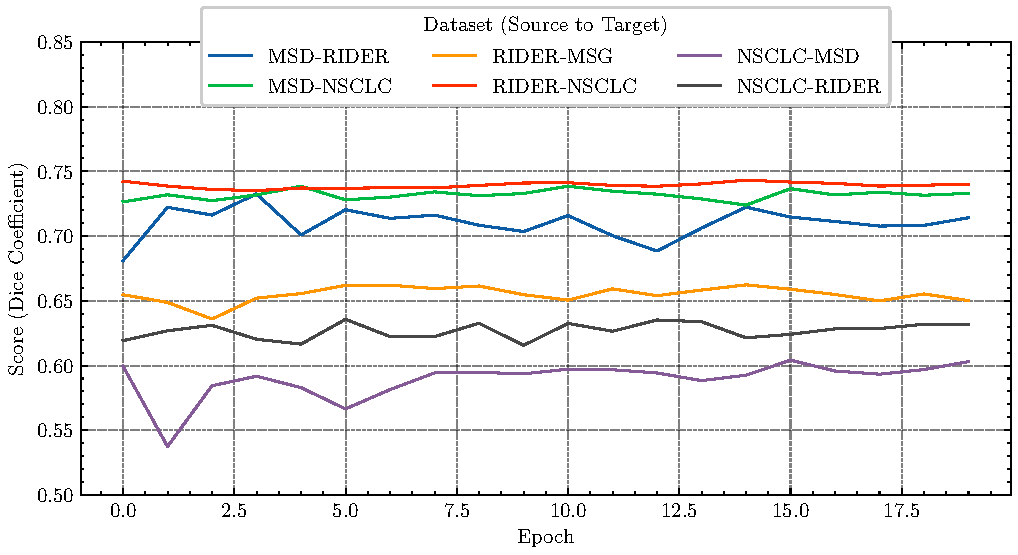
\includegraphics[width=0.95\textwidth]{fig/result/unetr_uda_val.pdf}
    \caption{The validation score chart for six dataset pairs in \acrshort{uda} framework based on \acrshort{unetr}.}
    \label{fig:unetr_uda_val}
\end{figure}

\subsection{Visualization Result}
As the original medical \acrshort{ct} volumes are through data preprocessing and augmentation, it is hard for the outputs of the model to be converted to a standard medical segmentation format (i.e. \acrshort{nifti} or \acrshort{dcmqi}) for further 3D model reconstruction. Fig \ref{fig:visual_seg} and Fig \ref{fig:visual_uda} show two slices with different states for model performance display in both segmentation model and \acrshort{uda} framework.

\begin{figure}[!htb]
   \begin{minipage}{0.48\textwidth}
     \centering
     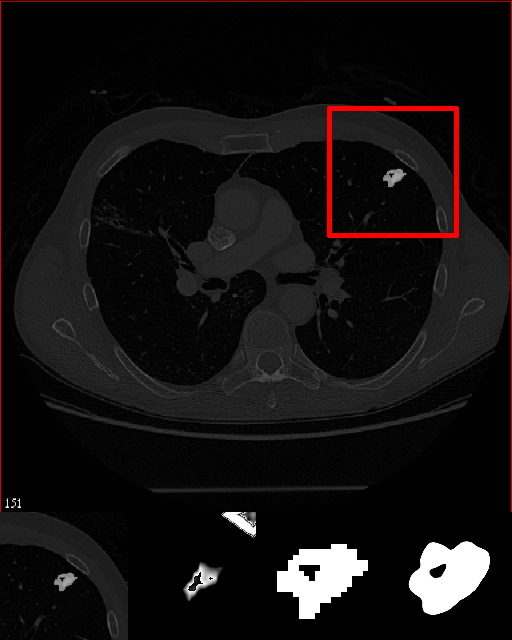
\includegraphics[width=.9\linewidth]{fig/result/visual_seg.png}
     \caption{The original segmentation result of "lung\_070.nii.gz" in the \acrshort{msd} dataset at frame 151 (from left to right, they are origin, preprocessed, label, and prediction).}\label{fig:visual_seg}
   \end{minipage}\hfill
   \begin{minipage}{0.48\textwidth}
     \centering
     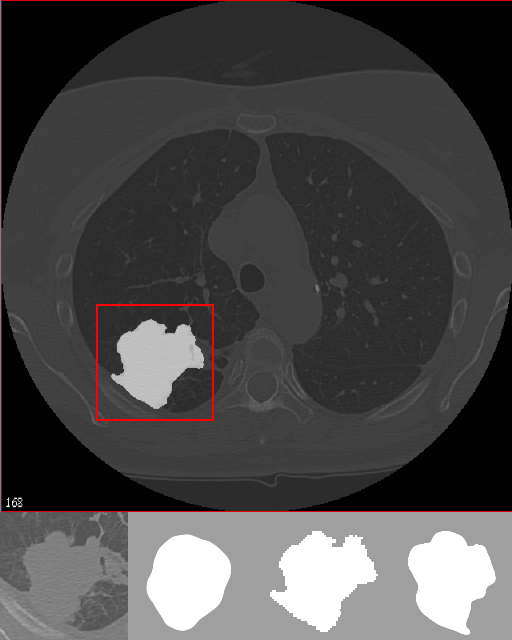
\includegraphics[width=.9\linewidth]{fig/result/visual_uda.png}
     \caption{The domain adaptation segmentation result of “RIDER-1129164940" in the \acrshort{rider} dataset at frame 168 (from left to right, they are origin, reconstruction, label, and prediction).
}\label{fig:visual_uda}
   \end{minipage}
\end{figure}

\chapter{Conclusion and Future Work}
\section{Conclusion}
In conclusion, the framework based on segmentation and shaping models can improve the model performance on unlabelled datasets by unsupervised domain adaptation. The Dice gap between a certain method and the upper bound is around 2\% in most cases. The 3D \acrshort{unet} with simple network architecture trained on the relatively abundant datasets \acrshort{rider} reaches the highest scores among the current results, which satisfies the weakness of \acrshort{vit} in labelled dataset shortage. In the small dataset \acrshort{nsclc}, the model pre-trained on other datasets provide more accurate segmentation than the upper bound result trained by the same dataset.
\section{Future Work}
This project needs further modification and maintenance in the future. More datasets with different scanning styles, such as combination of \acrshort{ct} and \acrshort{mri}, will be collected to analyse the bottlenecks of the current network. Some state-of-the-art components and mechanisms will be introduced into the network to handle the possible drawbacks, including accuracy, training time, and model size. Statistics about comparison with other segmentation methods will be evaluated in the future work.


% 参考文献列表,请打开 reference.bib 文件添加 bibtex 格式的参考文献
\bibliographystyle{IEEEtranN}
\bibliography{reference} %
\addcontentsline{toc}{chapter}{Bibliography}

\begin{appendices}
\chapter{Charts}
\label{appendix:charts}

\section{3D \acrshort{unet} Segmentation}
\begin{figure}[!htb]
   \begin{minipage}{0.48\textwidth}
     \centering
     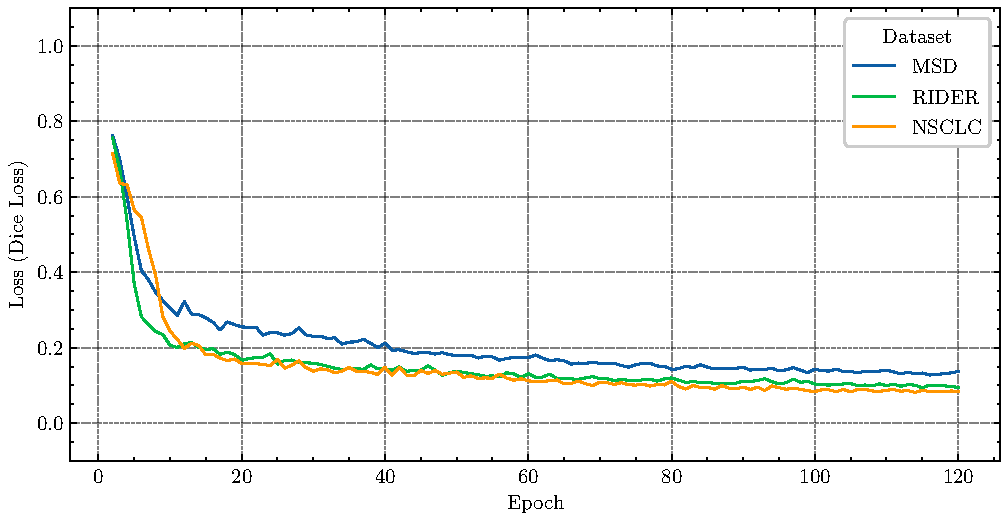
\includegraphics[width=\linewidth]{fig/result/seg_train.pdf}
     \caption{The training loss chart for three datasets in 3D \acrshort{unet} segmentation model.}\label{fig:app_seg_train}
   \end{minipage}\hfill
   \begin{minipage}{0.48\textwidth}
     \centering
     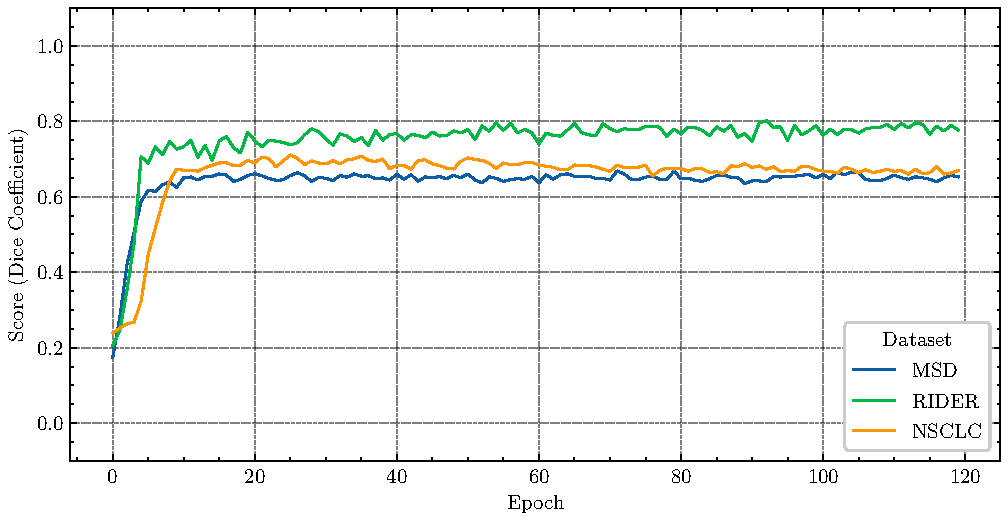
\includegraphics[width=\linewidth]{fig/result/seg_val.pdf}
     \caption{The validation score chart for three datasets in 3D \acrshort{unet} segmentation model.
}\label{fig:app_seg_val}
   \end{minipage}
\end{figure}

\section{\acrshort{unetr} Segmentation}
\begin{figure}[!htb]
   \begin{minipage}{0.48\textwidth}
     \centering
     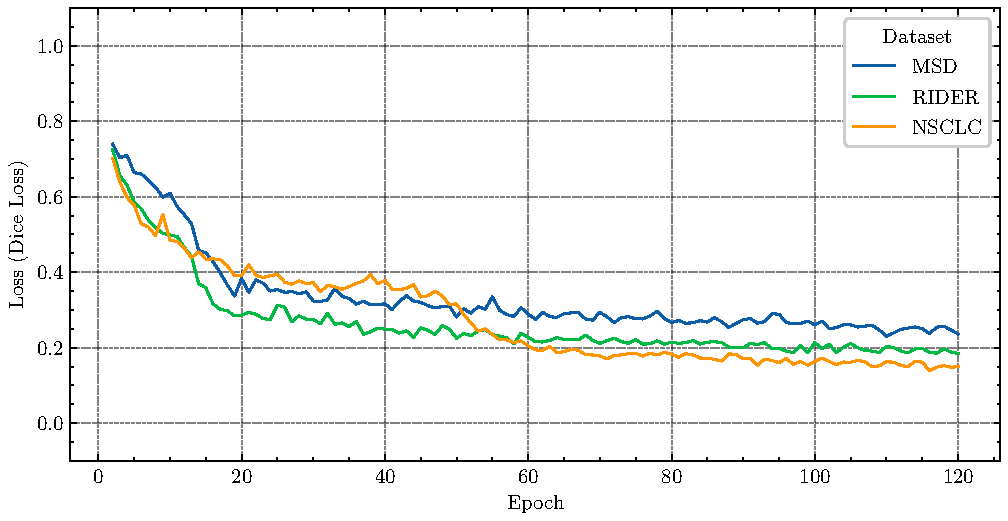
\includegraphics[width=\linewidth]{fig/result/unetr_train.pdf}
     \caption{The training loss chart for three datasets in \acrshort{unetr} segmentation model.}\label{fig:app_unetr_train}
   \end{minipage}\hfill
   \begin{minipage}{0.48\textwidth}
     \centering
     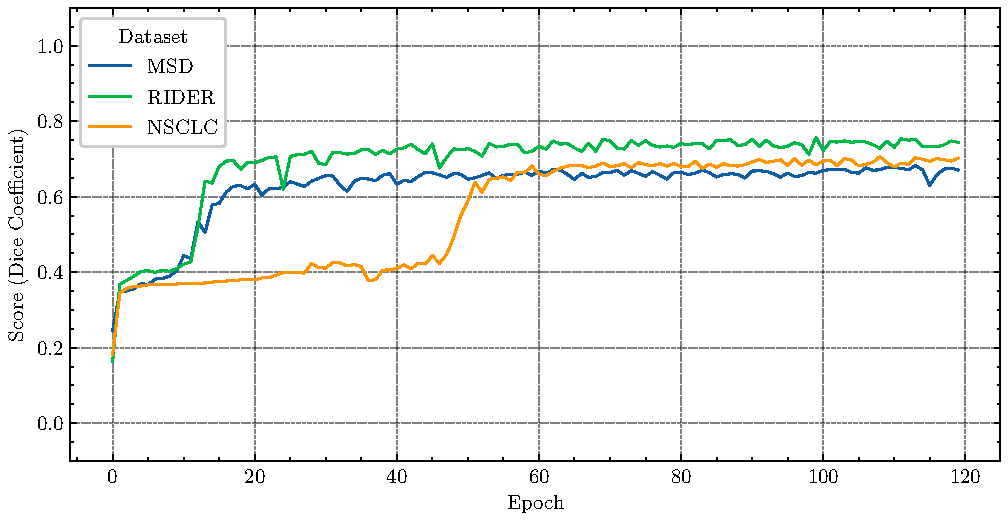
\includegraphics[width=\linewidth]{fig/result/unetr_val.pdf}
     \caption{The validation score chart for three datasets in \acrshort{unetr} segmentation model.
}\label{fig:app_unetr_val}
   \end{minipage}
\end{figure}

\clearpage

\section{\acrshort{vae} Shaping}
\begin{figure}[!htb]
   \begin{minipage}{0.48\textwidth}
     \centering
     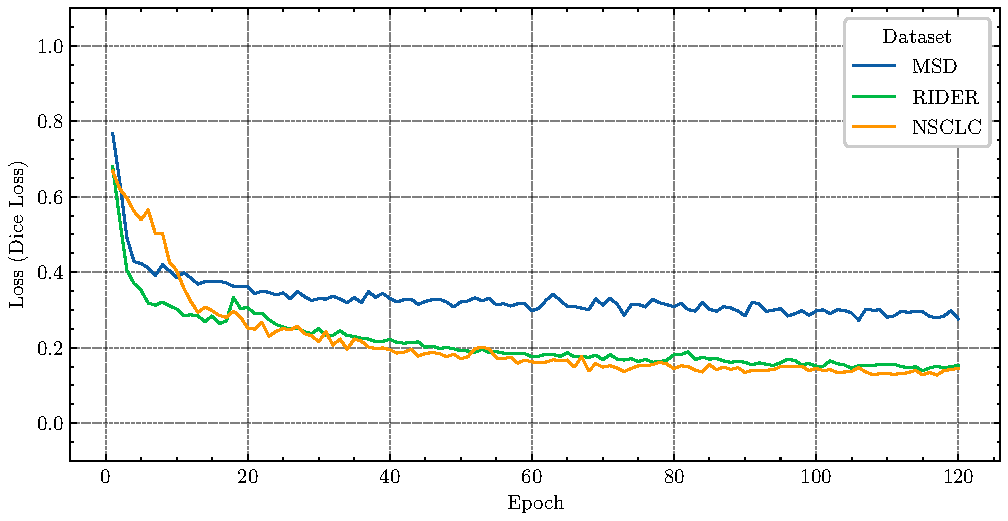
\includegraphics[width=\linewidth]{fig/result/vae_train.pdf}
     \caption{The training loss chart for three datasets in \acrshort{vae} shaping model.}\label{fig:app_vae_train}
   \end{minipage}\hfill
   \begin{minipage}{0.48\textwidth}
     \centering
     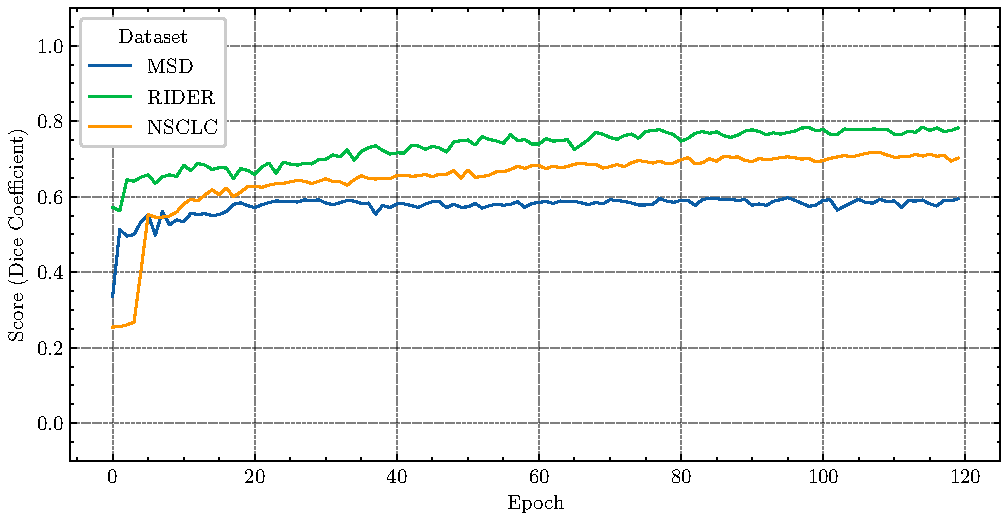
\includegraphics[width=\linewidth]{fig/result/vae_val.pdf}
     \caption{The validation score chart for three datasets in \acrshort{vae} shaping model.
}\label{fig:app_vae_val}
   \end{minipage}
\end{figure}

\section{3D \acrshort{unet} \acrshort{uda} framework}
\begin{figure}[!htb]
   \begin{minipage}{0.48\textwidth}
     \centering
     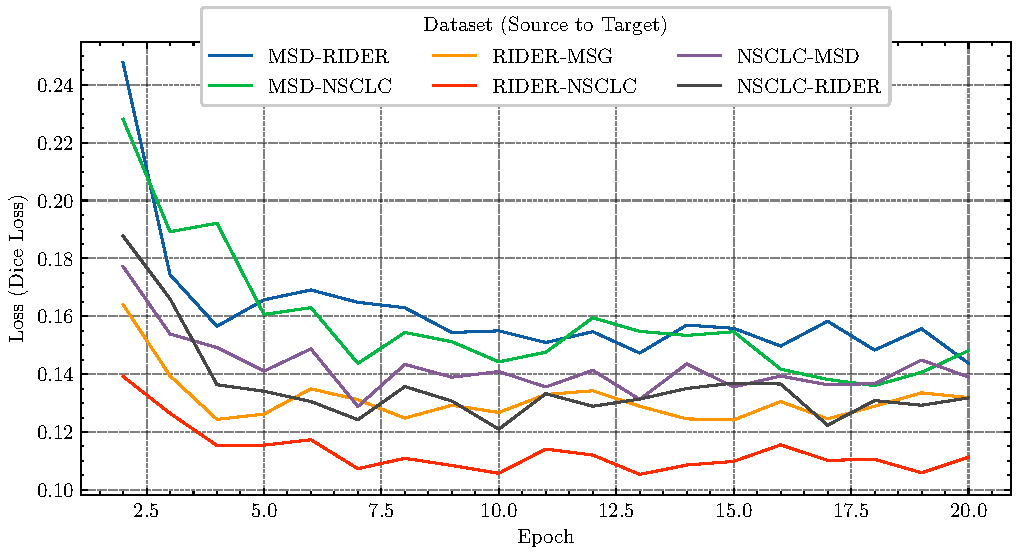
\includegraphics[width=\linewidth]{fig/result/seg_uda_train.pdf}
     \caption{The training loss chart for six dataset pairs in 3D \acrshort{unet} \acrshort{uda} framework.}\label{fig:app_seg_uda_train}
   \end{minipage}\hfill
   \begin{minipage}{0.48\textwidth}
     \centering
     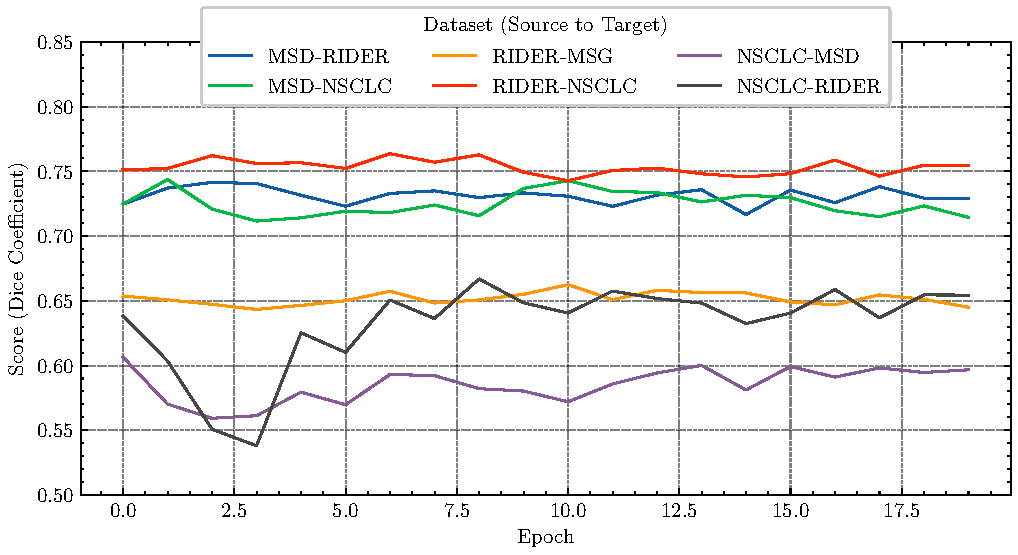
\includegraphics[width=\linewidth]{fig/result/seg_uda_val.pdf}
     \caption{The validation score chart for six dataset pairs in 3D \acrshort{unet} \acrshort{uda} framework.
}\label{fig:app_seg_uda_val}
   \end{minipage}
\end{figure}

\section{\acrshort{unetr} \acrshort{uda} framework}
\begin{figure}[!htb]
   \begin{minipage}{0.48\textwidth}
     \centering
     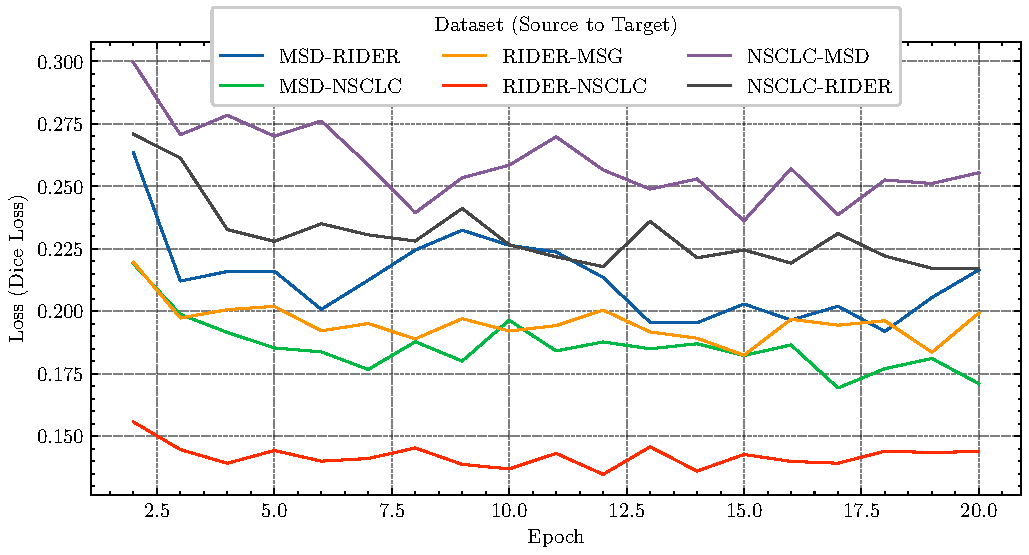
\includegraphics[width=\linewidth]{fig/result/unetr_uda_train.pdf}
     \caption{The training loss chart for six dataset pairs in \acrshort{unetr} \acrshort{uda} framework.}\label{fig:app_unetr_uda_train}
   \end{minipage}\hfill
   \begin{minipage}{0.48\textwidth}
     \centering
     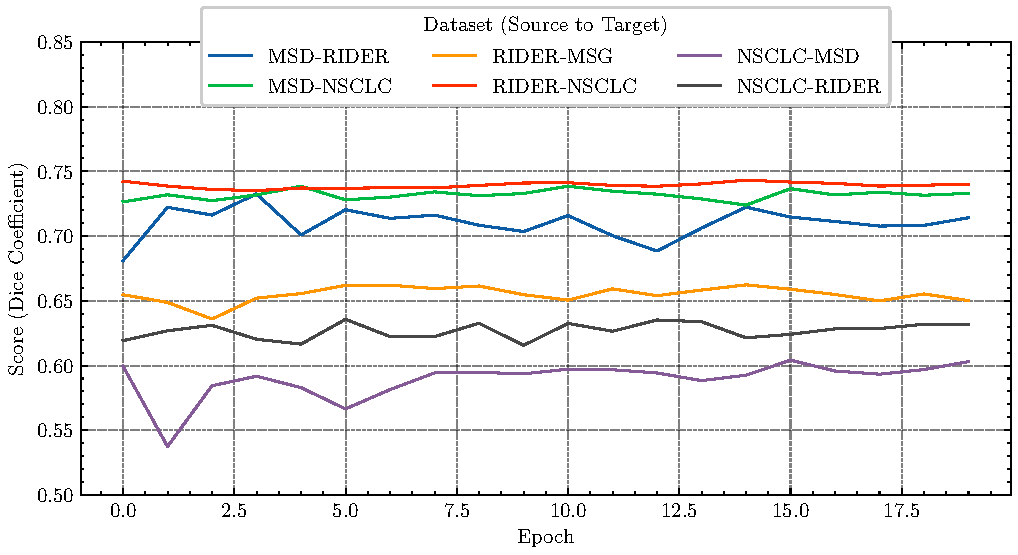
\includegraphics[width=\linewidth]{fig/result/unetr_uda_val.pdf}
     \caption{The validation score chart for six dataset pairs in \acrshort{unetr} \acrshort{uda} framework.
}\label{fig:app_unetr_uda_val}
   \end{minipage}
\end{figure}

\chapter{Project Code}
\section{dcm\_to\_nii.py}
\lstinputlisting[language=Python]{code/dcm_to_nii.py}
\clearpage
\section{data\_process.py}
\lstinputlisting[language=Python]{code/data_process.py}
\clearpage
\section{main\_source.py}
\lstinputlisting[language=Python]{code/main_source.py}
\clearpage
\section{main\_target.py}
\lstinputlisting[language=Python]{code/main_target.py}
\clearpage
\section{models.py}
\lstinputlisting[language=Python]{code/models.py}
\clearpage
\section{utils.py}
\lstinputlisting[language=Python]{code/utils.py}
\end{appendices}
\end{document}